\newpage
\chapter{Element Atlas}

\section{Matrices}

\textbf{The inversion formula for 3x3 matrix:}

\begin{eqarray}
    \m{A} &=
    \begin{bmatrix}
        a_{11} & a_{12} & a_{13}\\
        a_{21} & a_{22} & a_{23}\\
        a_{31} & a_{32} & a_{33}
    \end{bmatrix}\\
    \m{A}^{-1} &= \frac{1}{\vert \m{A} \vert}
    \begin{bmatrix}
        A_{11} & A_{12} & A_{13}\\
        A_{21} & A_{22} & A_{23}\\
        A_{31} & A_{32} & A_{33}
    \end{bmatrix}\\
\end{eqarray}

where:
\begin{eqarray}
    A_{11} &= a_{22} a_{33} - a_{23} a_{32}\\
    A_{22} &= a_{33} a_{11} - a_{31} a_{13}\\
    A_{33} &= a_{11} a_{22} - a_{12} a_{21}\\
    A_{12} &= a_{23} a_{31} - a_{21} a_{33}\\
    A_{23} &= a_{31} a_{12} - a_{32} a_{11}\\
    A_{31} &= a_{12} a_{23} - a_{13} a_{22}\\
    A_{21} &= a_{32} a_{13} - a_{12} a_{33}\\
    A_{32} &= a_{13} a_{21} - a_{23} a_{11}\\
    A_{13} &= a_{21} a_{22} - a_{31} a_{22}\\
    \vert A_{13} \vert &= a_{11} A_{11} + a_{12} A_{21} + a_{13} A_{31}
\end{eqarray}


\section{Numerical Integration}

\begin{bbox}
    \textbf{Note:}

    \textbf{Quadrature} is another term for \textbf{Numerical Integration}.
\end{bbox}


\subsection{Newton-Cotes quadrature}
In the most obvious procedure, points at which the function is to be formed are
determined \textit{a priori} - usually at equal intervals - and a polynomial
passed through the values of the function at these points and exactly integrated.

As $ n $ values define a polynomial of degree $ n - 1 $, the errors will be
of the order $ O(h^n) $ where $ h $ is the element size. This leads to the
well-known \textbf{Newton-Cotes} \'quadrature formulae\'. The integrals can be
written as:

\begin{equation}
    I = \int_{-1}^{1} f(\xi) d\xi = \sum_1^n H_i f(\xi_i)
\end{equation}

for the range of integration between $ -1 $ and $ +1 $. For example, if $ n = 2 $,
we have the well-known trapezoidal rule:

\begin{equation}
    I = f(-1) + f(1)
\end{equation}

for $ n = 3 $, the well-known \textbf{Simpson} one-third rule:

\begin{equation}
    I = \frac{1}{3} \left[ f(-1) + 4f(0) + f(1) \right]
\end{equation}

and for $ n = 4 $:

\begin{equation}
    I = \frac{1}{4} \left[f(-1) + 3f(-\frac{1}{3}) + 3f(\frac{1}{3}) + f(1) \right]
\end{equation}


\subsection{Gauss quadrature}

If in place of specifying the position of sampling points \textit{a priori} we
allow these to be located at points to be determined so as to aim for best
accuracy, then for a given number of sampling points increased accuracy can be
obtained. Indeed, if we again consider:

\begin{equation}
    I = \int_{-1}^{1} f(\xi) d\xi = \sum_1^n H_i f(\xi_i)
\end{equation}

and again assume a polynomial expression, it is easy to see that for $ n $ sampling
points we have $ 2n $ unknowns ($H_i$ and $\xi_i$) and hence a polynomial of degree
$ 2n-1 $ could be constructed and exactly integrated. The error is thus of order
$ O(h^{2n}) $.

The simultaneous equations involved are difficult to solve, but some mathematical
manipulation will show that the solution can be obtained explicitely in terms
of \textbf{Legendre polynomials}. Thus this particular process is frequently known
as \textbf{Gauss-Legendre} quadrature.

For purposes of finite elements analysis complex calculations are involved in
determining the values of $ f $, the function to be integratet. Thus the
Gauss-type processes, requiring the least number of such evaluations, are ideally
suited and are mostly used exvlusively.

Other expresssions for integration of functions of the type

\begin{equation}\label{leggaus}
    I = \int_{-1}^{1} w(\xi) f(\xi) d\xi = \sum_{1}^{n} H_i f(\xi_i)
\end{equation}

can be derived for prescribed forms of $ w(\xi) $, again integrating up to a certain
order of accuracy a polynomial expansion of $ f(\xi) $.


\subsection{Linear and Quadrilateral Elements}

\subsubsection{For 1D:}

\begin{equation}
    I = \int_{-1}^{1} f(\xi) d\xi = \sum_1^n H_i f(\xi_i)
\end{equation}


\subsubsection{For 2D:}

The most obvious way of obtaining the integral:

\begin{equation}
    I = \int_{-1}^{1} \int_{-1}^{1} f(\xi, \eta) d\xi d\eta
\end{equation}

Is to first evaluate the inner integral keeping $ \eta $ constant, i.e.:

\begin{equation}
    \int_{-1}^{1}f(\xi, \eta) d\xi = \sum_{j=1}^n H_j f(\xi_i, \eta) = \psi(\eta)
\end{equation}

Evaluating the outer integral in a similar manner, we have:

\begin{eqarray}
    I = \int_{-1}^{1} \psi(\eta) d\eta
    &= \sum_{i=1}^n H_i \psi(\eta_i)\\
    &= \sum_{i=1}^n H_i \sum_{j=1}^n H_j f(\xi_i,\eta_i)\\
    &= \sum_{i=1}^n \sum_{j=1}^n H_i H_j f(\xi_j,\eta_i)
\end{eqarray}

\subsubsection{For 3D:}
For a 3D element we have similarly:

\begin{eqarray}
    I &= \int_{-1}^{1} \int_{-1}^{1} \int_{-1}^{1} f(\xi, \eta, \mu) d\xi d\eta d\mu\\
    &= \sum_{i=1}^n \sum_{j=1}^n \sum_{k=1}^n H_i H_j f(\xi_i,\eta_j,\mu_k)
\end{eqarray}

In the above, the number of integrating points in each direction was assumed to be
the same. Clearly this is not necessary and on occasion it may be an advantage to
use different numbers in each direction of integration.

\begin{figure}[ht]
    \centering
    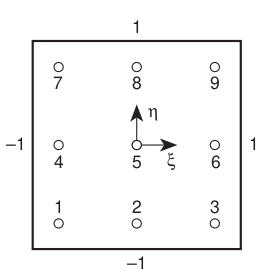
\includegraphics[width=0.25\textwidth]{img/quad_interpolation_3.png}
    \caption{Integration points for $ n = 3 $ in a square region. Exact for a
    polynomial of fifth order in each direction}
    \label{fig:quad-interpolation-3-png}
\end{figure}

\begin{table}
    \centering
    \renewcommand{\arraystretch}{1.25}
    \begin{tabular}{||c c c||}
        \hline
        \hline
        integration point & polynomial order & weight\\
        \hline
        \hline
        0 & n = 1 & 2.0\\
        \hline
        \begin{tabular}{c}
            $ -1/\sqrt{3} $ \\
            $ 1/\sqrt{3} $
        \end{tabular} & n = 2 &
        \begin{tabular}{c}
            1.0 \\
            1.0
        \end{tabular} \\
        \hline
        \begin{tabular}{c}
            $ -\sqrt{0.6} $ \\
            $ 0.0 $ \\
            $ \sqrt{0.6} $
        \end{tabular} & n = 3 &
        \begin{tabular}{c}
            $ 5/9 $ \\
            $ 8/9 $ \\
            $ 5/9 $
        \end{tabular} \\
        \hline
        \begin{tabular}{c}
            -0.861 136 311 594 953 \\
            -0.339 981 043 584 856 \\
             0.339 981 043 584 856 \\
             0.861 136 311 594 953 \\
        \end{tabular} & n = 4 &
        \begin{tabular}{c}
            0.347 854 845 137 454 \\
            0.652 145 154 862 546 \\
            0.652 145 154 862 546 \\
            0.347 854 845 137 454 \\
        \end{tabular} \\
        \hline
        \begin{tabular}{c}
            -0.906 179 845 938 664 \\
            -0.538 469 310 105 683 \\
             0.000 000 000 000 000 \\
             0.538 469 310 105 683 \\
             0.906 179 845 938 664 \\
        \end{tabular} & n = 5 &
        \begin{tabular}{c}
            0.236 926 885 056 189 \\
            0.478 628 670 499 366 \\
            0.568 888 888 888 889 \\
            0.478 628 670 499 366 \\
            0.236 926 885 056 189 \\
        \end{tabular} \\
        \hline
        \begin{tabular}{c}
            -0.932 469 514 203 152 \\
            -0.661 209 386 466 265 \\
            -0.238 619 186 083 197 \\
             0.238 619 186 083 197 \\
             0.661 209 386 466 265 \\
             0.932 469 514 203 152 \\
        \end{tabular} & n = 6 &
        \begin{tabular}{c}
            0.171 324 492 379 170 \\
            0.360 761 573 048 139 \\
            0.467 913 934 572 691 \\
            0.467 913 934 572 691 \\
            0.360 761 573 048 139 \\
            0.171 324 492 379 170 \\
        \end{tabular} \\
        \hline
        \begin{tabular}{c}
            -0.949 107 912 342 759 \\
            -0.741 531 185 599 394 \\
            -0.405 845 151 377 397 \\
             0.000 000 000 000 000 \\
             0.405 845 151 377 397 \\
             0.741 531 185 599 394 \\
             0.949 107 912 342 759 \\
        \end{tabular} & n = 7 &
        \begin{tabular}{c}
            0.129 484 966 168 870 \\
            0.279 705 391 489 277 \\
            0.381 830 050 505 119 \\
            0.471 959 183 673 469 \\
            0.381 830 050 505 119 \\
            0.279 705 391 489 277 \\
            0.129 484 966 168 870 \\
        \end{tabular} \\
        \hline
        \hline
    \end{tabular}
    \caption{Gauss-Legendre Integration Points and Weights}
\end{table}

\begin{bbox}
    To get the \textbf{Gauss-Legendre} points and weights in python use:

    \begin{python}
import numpy as np

# number of integration points
N = 3

points, weights = np.polynomial.legendre.leggauss(N)
    \end{python}
\end{bbox}


\newpage
\subsection{Triangular and Tetrahedral elements:}

\subsubsection{2D}
For a triangle, in terms of the \textbf{area coordinates} the integrals are of the
form:

\begin{equation}
    I = \int_{0}^{1} \int_{0}^{1-\xi} f(\xi, \eta, \mu) d\eta d\xi, \quad
    \mu = 1 - \xi - \eta
\end{equation}

Once again we could use $ n $ Gauss points and arrive at a summation expression of
the type used in the previous section. However, the limits of integration now
involve the variable itself and it is convenient to use alternative sampling points
for the second integration by use of a special Gauss expression for integrals of
the type given by equation \eqref{leggaus} in which $ w $ is a linear function.
These have been devised by \textit{Radau} and used successfully in finite element context.
It is, however, much more desirable (and aesthetically pleasing) to use special
formulae in which no bias is given to any of the natural coordinates ($\xi, \eta, \mu$).
Such formulae were first derived by \textit{Hammer et al.} and \textit{Felippa}
and a series of necessary sampling points and weights.

\newpage
\begin{table}[h!]
    \centering
    \renewcommand{\arraystretch}{1.25}
    % \small
    % \scriptsize
    \scalebox{0.80}{
    \begin{tabular}{||c c c c c c||}
        \hline
        \hline
        Order & Figure & Error & Points &
        \begin{tabular}{c} Triangular\\Coordinates\end{tabular} & Weights\\
        \hline
            Linear &
            \begin{tabular}{c}
                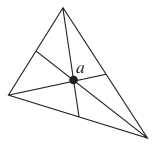
\includegraphics[width=0.20\textwidth]{img/tria_linear.png}\\
            \end{tabular}
            & $ R = O(h^2) $ & a & $ \frac{1}{3}, \frac{1}{3}, \frac{1}{3} $ & 1\\
        \hline
            Quadratic &
            \begin{tabular}{c}
                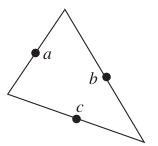
\includegraphics[width=0.20\textwidth]{img/tria_quadratic.png}
            \end{tabular}
            & $ R = O(h^3) $ & \begin{tabular}{c}
                a \\
                b \\
                c \\
            \end{tabular} & \begin{tabular}{c}
                $ \frac{1}{2}, \frac{1}{2} , 0 $ \\
                $ 0, \frac{1}{2}, \frac{1}{2} $ \\
                $ \frac{1}{2}, 0, \frac{1}{2} $ \\
            \end{tabular} & \begin{tabular}{c}
                $ \frac{1}{3} $ \\
                $ \frac{1}{3} $ \\
                $ \frac{1}{3} $ \\
            \end{tabular}\\
        \hline
            Cubic &
            \begin{tabular}{c}
                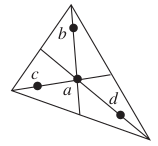
\includegraphics[width=0.20\textwidth]{img/tria_cubic.png}
            \end{tabular}
            & $ R = O(h^4) $ & \begin{tabular}{c}
                a \\
                b \\
                c \\
                d \\
            \end{tabular} & \begin{tabular}{c}
                $ \frac{1}{3}, \frac{1}{3} , \frac{1}{3} $ \\
                $ 0.6, 0.2, 0.2 $ \\
                $ 0.2, 0.6, 0.2 $ \\
                $ 0.2, 0.2, 0.6 $ \\
            \end{tabular} & \begin{tabular}{c}
                $ -\frac{27}{48} $ \\
                $ \frac{25}{48} $ \\
                $ \frac{25}{48} $ \\
                $ \frac{25}{48} $ \\
            \end{tabular}\\
        \hline
            Quintic &
            \begin{tabular}{c}
                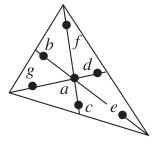
\includegraphics[width=0.20\textwidth]{img/tria_quintic.png}
            \end{tabular}
            & $ R = O(h^6) $ & \begin{tabular}{c}
                a \\
                b \\
                c \\
                d \\
                e \\
                f \\
                g \\
            \end{tabular} & \begin{tabular}{c}
                $ \frac{1}{3}, \frac{1}{3} , \frac{1}{3} $ \\
                $ \alpha_1, \beta_1, \beta_1 $ \\
                $ \beta_1, \alpha_1, \beta_1 $ \\
                $ \beta_1, \beta_1, \alpha_1 $ \\
                $ \alpha_2, \beta_2, \beta_2 $ \\
                $ \beta_2, \alpha_2, \beta_2 $ \\
                $ \beta_2, \beta_2, \alpha_2 $ \\
            \end{tabular} & \begin{tabular}{c}
                $ 0.225 000 000 0 $ \\
                $ 0.132 394 152 7 $ \\
                $ 0.132 394 152 7 $ \\
                $ 0.132 394 152 7 $ \\
                $ 0.125 939 180 5 $ \\
                $ 0.125 939 180 5 $ \\
                $ 0.125 939 180 5 $ \\
            \end{tabular}\\
            & & & \multicolumn{2}{l}{\begin{tabular}{l}
                with: \\
                $ \alpha_1 = $ 0.059 715 871 7 \\
                $ \beta_1 = $ 0.470 142 064 1 \\
                $ \alpha_2 = $ 0.797 426 985 3 \\
                $ \beta_2 = $ 0.101 286 507 3 \\
            \end{tabular}} & \\
        \hline
        \hline
    \end{tabular}}
    \caption{Triangular Element integration points and weights}
\end{table}


\newpage
\begin{table}[h!]
    \centering
    \renewcommand{\arraystretch}{1.25}
    % \small
    % \scriptsize
    \scalebox{0.80}{
    \begin{tabular}{||c c c c c c||}
        \hline
        \hline
        Order & Figure & Error & Points &
        \begin{tabular}{c} Tetrahedral\\Coordinates\end{tabular} & Weights\\
        \hline
            Linear &
            \begin{tabular}{c}
                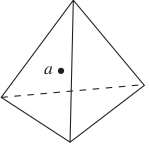
\includegraphics[width=0.20\textwidth]{img/tetra_linear.png}\\
            \end{tabular}
            & $ R = O(h^2) $ & a & $ \frac{1}{4}, \frac{1}{4}, \frac{1}{4}, \frac{1}{4} $ & 1\\
        \hline
            Quadratic &
            \begin{tabular}{c}
                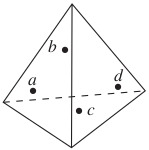
\includegraphics[width=0.20\textwidth]{img/tetra_quadratic.png}
            \end{tabular}
            & $ R = O(h^6) $ & \begin{tabular}{c}
                a \\
                b \\
                c \\
                d \\
            \end{tabular} & \begin{tabular}{c}
                $ \alpha, \beta, \beta, \beta $ \\
                $ \beta, \alpha, \beta, \beta $ \\
                $ \beta, \beta, \alpha, \beta $ \\
                $ \beta, \beta, \beta, \beta $ \\
            \end{tabular} & \begin{tabular}{c}
                $ \frac{1}{4} $ \\
                $ \frac{1}{4} $ \\
                $ \frac{1}{4} $ \\
                $ \frac{1}{4} $ \\
            \end{tabular}\\
            & & & \multicolumn{2}{l}{\begin{tabular}{l}
                with: \\
                $ \alpha = $ 0.585 410 20 \\
                $ \beta = $ 0.138 196 60 \\
            \end{tabular}} & \\
        \hline
            Cubic &
            \begin{tabular}{c}
                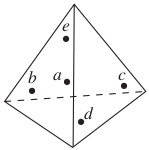
\includegraphics[width=0.20\textwidth]{img/tetra_cubic.png}
            \end{tabular}
            & $ R = O(h^4) $ & \begin{tabular}{c}
                a \\
                b \\
                c \\
                d \\
                e \\
            \end{tabular} & \begin{tabular}{c}
                $ \frac{1}{4}, \frac{1}{4}, \frac{1}{4}, \frac{1}{4} $ \\
                $ \frac{1}{2}, \frac{1}{6}, \frac{1}{6}, \frac{1}{6} $ \\
                $ \frac{1}{6}, \frac{1}{2}, \frac{1}{6}, \frac{1}{6} $ \\
                $ \frac{1}{6}, \frac{1}{6}, \frac{1}{2}, \frac{1}{6} $ \\
                $ \frac{1}{6}, \frac{1}{6}, \frac{1}{6}, \frac{1}{2} $ \\
            \end{tabular} & \begin{tabular}{c}
                $ -\frac{4}{5} $ \\
                $ \frac{9}{20} $ \\
                $ \frac{9}{20} $ \\
                $ \frac{9}{20} $ \\
                $ \frac{9}{20} $ \\
            \end{tabular}\\
        \hline
        \hline
    \end{tabular}}
    \caption{Tetrahedral Element integration points and weights}
\end{table}



\newpage
\section{General Element Matrices Procedure}
The procedure to generate any element stiffness, mass and load matrices can
be generalised to the following steps:

\begin{enumerate}
    \item Create Element domain in natural coordinates:
        \begin{itemize}
            \item $ -1 $ to $ 1 $ for quadrilateral elements
            \item $ 0 $ to $ 1 $ for triangular and linear elements
        \end{itemize}

    \item select the number of Gauss points based on the order of the element
        \begin{itemize}
            \item $ 2 $ for linear elements
            \item $ 3 $ for quadratic elements
        \end{itemize}

        Example:
        \begin{python}
import numpy as np
gp, gw = np.polynomial.legendre.leggauss(3)
        \end{python}

    \item Generate the shape functions $ \m{N}_n^e $ in natural coordinates
        based on the number of Gauss points, dimension of the element and its domain.

        The $ \m{N}_n^e $ matrix has the dimensions of:
        \begin{itemize}
            \item number of integration points = number of rows
            \item number of shape functions = number of columns
        \end{itemize}

        Therefore:

        \begin{equation}
            \m{N}_n^e = \begin{bmatrix}
                N_{1,1}^e & \dots & N_{n,1}^e\\
                \vdots & \vdots & \vdots\\
                N_{1,m}^e & \dots & N_{n,m}^e
            \end{bmatrix}
        \end{equation}
         where $ 1 \dots m $ are the integration points and $ 1 \dots n $ are the shape
         functions.

    \item Transform the shape functions from natural coordinates to global coordinates
        \begin{eqarray}
            \m{N}_g^e &= \m{N}_n^e \m{x}^e\\
            \m{N}_g^e &= \begin{bmatrix}
                N_{1,1}^e(\xi) & \dots & N_{n,1}^e(\xi)\\
                \vdots & \vdots & \vdots\\
                N_{1,m}^e(\xi) & \dots & N_{n,m}^e(\xi)
            \end{bmatrix}
            \begin{bmatrix}
                x_1 & y_1 & z_1\\
                \vdots & \vdots & \vdots\\
                x_n & y_n & z_n
            \end{bmatrix}
        \end{eqarray}

        The $ \m{x}^e $ matrix is a matrix of global coordinates of the element nodes.

        The resulting matrix has the dimension of:
        \begin{itemize}
            \item number of integration points = number of rows
            \item number of coordinates = number of columns (3D = 3, 2D = 2)
        \end{itemize}

    \item Generate the shape functions derivatives $ \m{B}_n^e $
        in natural coordinates

        The shape functions derivatives matrix has 3 dimensions being
        \textit{number of integration points} $\times$ \textit{number of natural coordinates}
        $\times$ \textit{number of shape functions}

    \item Create the Matrix of Jacobians from the shape functions derivatives:
        \begin{equation}
            \m{J} = \m{B}_n^e \m{x}^e
        \end{equation}

        The Matrix of Jacobians has the dimension of \textit{number of integration points}
        $\times$ \textit{number of global coordinates}
        $\times$ \textit{number of global coordinates}, where number of global coordinates
        means 2 for 2D and 3 for 3D problem.

    \item Get the Matrix of Jacobian determinants and an inverse Jacobian:
        \begin{equation}
            \m{J}^{-1}\\
            \m{J}_d = det \m{J}
        \end{equation}

        Example:
        \begin{python}
d_jacobi = np.linalg.det(jacobi)
i_jacobi = np.linalg.inv(jacobi)
        \end{python}

        The Jacobian determinant is computed for each integration point and has a dimension
        of \textit{number of integration points} $\times$ \textit{1}

        The inverse Jacobian has the same dimension as the Jacobian (\textbf{must have})

    \item Transform the shape function derviatives from natural coordinates to
        global coordinates
        \begin{equation}
            \m{B}_g^e = \m{J}^{-1} \m{B}_n^e
        \end{equation}

    \item Create the Material Stiffness matrix $ \m{C} $

    \item Finally for each integration point:

        3D:
        \begin{eqarray}
            \m{B}_{i,x}^e &= \m{B}_g(i, 0) \\
            \m{B}_{i,y}^e &= \m{B}_g(i, 1) \\
            \m{B}_{i,z}^e &= \m{B}_g(i, 2)\\
        \end{eqarray}

        where $ \m{B}_{i,x}^e $,  $ \m{B}_{i,y}^e $ and  $ \m{B}_{i,z}^e $
        are vectors of legth = \textit{number of shape functions}

        Then matrix $ \m{B} $ is:

        \begin{equation}
            \m{B}_i = \begin{bmatrix}
                \m{B}_{i,x}^e & \m{0} & \m{0}\\
                \m{0} & \m{B}_{i,y}^e & \m{0}\\
                \m{0} & \m{0} & \m{B}_{i,z}^e \\
                \m{B}_{i,y}^e & \m{B}_{i,x}^e & \m{0}\\
                \m{0} & \m{B}_{i,z}^e & \m{B}_{i,y}^e \\
                \m{B}_{i,z}^e & \m{0} & \m{B}_{i,x}^e
            \end{bmatrix}
        \end{equation}

        and matrix $ \m{N} $ is:

        \begin{equation}
            \m{N}_i = \begin{bmatrix}
                \m{N}_{n,i}^e & \m{0} & \m{0}\\
                \m{0} & \m{N}_{n,i}^e & \m{0}\\
                \m{0} & \m{0} & \m{N}_{n,i}^e
            \end{bmatrix}
        \end{equation}

        where $ \m{0} $ is a zero vector of length = \textit{number of shape functions}
        and $ \m{N}_{n,i}^e $ is a vector of shape functions in natural coordinates
        pertaining to the $i$-th integration point.

        Then:

        \begin{enumerate}
            \item \begin{equation}
                    \m{K}_i^e = \m{B}_i^T \m{C} \m{B}_i \ det \m{J}_i
                    w_i
                  \end{equation}

            \item \begin{equation}
                    \m{M}_i^e = \rho \m{N}_i^T \m{N}_i \ det \m{J}_i
                    w_i
                  \end{equation}
            \item \begin{equation}
                    \m{F}_i^e = \m{N}_i^T \m{F} \ det \m{J}_i
                    w_i
                  \end{equation}

                  where $ \m{F} = \begin{bmatrix}f_x \\ f_y \\ f_z\end{bmatrix} $
        \end{enumerate}

        where $ w_i $ is the multiple of gaussian weights for the respective
        integration point (for 3D case brick where the natural coordinates
        are $ \xi $, $ \eta $, $ \mu $ the $ w_i = w_{\xi_i} w_{\eta_i} w_{\mu_i} $

    \item Finally:
        \begin{enumerate}
            \item \begin{equation}
                    \m{K}^e = \sum_{i=1}^n \m{K}_i^e
                \end{equation}

            \item \begin{equation}
                    \m{M}^e = \sum_{i=1}^n \m{M}_i^e
                \end{equation}

            \item \begin{equation}
                    \m{F}^e = \sum_{i=1}^n \m{F}_i^e
                \end{equation}
        \end{enumerate}
\end{enumerate}


\newpage
\section{ROD}

\subsection{Element Formulation}
The \textbf{rod} element is a 1-D linear element. It has 2 nodes, and 3 dofs for
each node $ u_x, u_y, u_y $ (or $ u, v, w $). Rotation \textbf{DOF}s are not
constrained.

\subsubsection{Natural coordinates}
The natural coordinate $ \xi $ of the \textbf{ROD} element goes from $ 0 $ to $ 1 $.
The 2-noded rod element is defined by:

\begin{equation}
    \begin{bmatrix}
        1 \\
        x \\
        y \\
        z \\
        u_x \\
        u_y \\
        u_z \\
    \end{bmatrix}
    = \begin{bmatrix}
        1 & 1 \\
        x_1 & x_2 \\
        y_1 & y_2 \\
        z_1 & z_2 \\
        u_{x1} & u_{x2} \\
        u_{y1} & u_{y2} \\
        u_{z1} & u_{z2} \\
    \end{bmatrix}
    \begin{bmatrix}
        N_1^e \\
        N_2^e \\
    \end{bmatrix}
\end{equation}

\subsubsection{Shape Functions}
The \textbf{ROD} natural coordinates are:

\begin{table}[ht]
    \centering
    \begin{tabular}{|c c |}
        \hline
        node & $\xi$ \\
        \hline
        1 & 0 \\
        2 & 1 \\
        \hline
    \end{tabular}\\
    \caption{ROD corners natural coordinates}
\end{table}

The shape functions are:

\begin{eqarray}
    N_1^e &= 1 - \xi \\
    N_2^e &= \xi \\
\end{eqarray}


\subsubsection{Partial Derivatives}
The shape function derivatives with respect to the natural coordinate:

\begin{eqarray}
    \frac{\partial N_1^e}{\partial \xi} &= -1 \\
    \frac{\partial N_2^e}{\partial \xi} &= \phantom{-}1 \\
\end{eqarray}

\subsubsection{The Jacobian}

The derivatives of the shape functions are given by the usual chain rule formula:
\begin{eqarray}
    \frac{\partial N_i^e}{\partial x} &= \frac{\partial N_i^e}{\partial \xi}
                                         \frac{\partial \xi}{\partial x} \\
    \frac{\partial N_i^e}{\partial y} &= \frac{\partial N_i^e}{\partial \xi}
                                         \frac{\partial \xi}{\partial y} \\
    \frac{\partial N_i^e}{\partial z} &= \frac{\partial N_i^e}{\partial \xi}
                                         \frac{\partial \xi}{\partial z} \\
\end{eqarray}

In matrix form:
\begin{equation}
    \begin{bmatrix}
        \frac{\partial N_i^e}{\partial x} \\
        \frac{\partial N_i^e}{\partial y} \\
        \frac{\partial N_i^e}{\partial z} \\
    \end{bmatrix}
    = \begin{bmatrix}
        \frac{\partial \xi}{\partial x} \\
        \frac{\partial \xi}{\partial y} \\
        \frac{\partial \xi}{\partial z} \\
    \end{bmatrix}
    \begin{bmatrix}
        \frac{\partial N_i^e}{\partial \xi} \\
    \end{bmatrix}
\end{equation}

The $ 3 \times 1 $ matrix above is $ \m{J}^{-1} $, the inverse of:
\begin{equation}
    \m{J} = \frac{\partial (x, y, z)}{\partial(\xi)} =
    \begin{bmatrix}
        \frac{\partial x}{\partial \xi} &
        \frac{\partial y}{\partial \xi} &
        \frac{\partial z}{\partial \xi} \\
    \end{bmatrix}
\end{equation}

Given the element coordinates the Jacobian can be computed:
\begin{equation}
    \m{J}_i = \begin{bmatrix}
        \frac{\partial N_i^e}{\partial \xi} &
        \frac{\partial N_i^e}{\partial \xi} &
        \frac{\partial N_i^e}{\partial \xi} \\
    \end{bmatrix}
    \begin{bmatrix}
        x_i \\
        y_i \\
        z_i \\
    \end{bmatrix}
\end{equation}

end then numerically inverted for $ \m{J}^{-1} $.

\begin{bbox}
    If the $ \m{J} $ is not a square matrix, then \textbf{Moore-Penrose pseudoinverse}
    applies:

    \begin{equation}
        \m{J}^{-1} = \m{J}^{+} = \left( \m{J}^T \m{J} \right)^{-1} \m{J}^T
    \end{equation}

    in python:

    \begin{minted}[linenos=true, xleftmargin=1cm]{python}
        import numpy as np

        J_i = np.linalg.pinv(J)
    \end{minted}

\end{bbox}

\begin{bbox}
    Assembling the \textbf{Jacobian} thegether gives essentially that for a 1D case

    \begin{equation}
        \m{J} = l
    \end{equation}

    and therefore:
    \begin{equation}
        \m{J}^{-1} = \frac{1}{l}
    \end{equation}

    \begin{equation}
        \det{J} = l
    \end{equation}
\end{bbox}

afterwards for each integration point:
\begin{equation}
    \m{N}^i_g = \m{N}^i \m{u}
\end{equation}

\begin{equation}
    \m{B}^i_g = {\m{J}^i}^{-1} \frac{\partial N}{\partial \xi}^i
\end{equation}

then:
\begin{eqarray}
    \m{K}^e &\eqp {\m{B}^i_g}^T \m{D} {\m{B}^i_g} \det \m{J}^i w^i \\
    \m{M}^e &\eqp \rho {\m{N}^i}^T {\m{N}^i} \det \m{J}^i w^i \\
    \m{F}^e &\eqp {\m{N}^i}^T \m{F} \det \m{J}^i w^i \\
\end{eqarray}





\subsection{Example 1D}
If assembling the element in local CSYS, then $ u_y = 0 $ and $ u_z = 0 $.
Simplifiying the equations gives that:
\begin{equation}
    \m{N} = \begin{bmatrix}
        N_1^e & N_2^e \\
    \end{bmatrix}
    = \begin{bmatrix}
        1 - \xi & \xi \\
    \end{bmatrix}
\end{equation}

and
\begin{equation}
    u^e(\xi) = \m{N} \begin{bmatrix}
        u_1^e \\
        u_2^e \\
    \end{bmatrix}
\end{equation}

shape function derivatives:
\begin{equation}
    \m{B} = \frac{\partial \m{N}}{\partial \xi} =
    \begin{bmatrix}
        -1 & 1 \\
    \end{bmatrix}
\end{equation}

the strain-displacement realtion is given by:
\begin{equation}
    \M{\epsilon} = \m{B} \m{u}
\end{equation}

Integrating the element at midpoint $ \xi = 0.5 $ with a weight of $ w = 1.0 $
(for interval $ \left< 0, 1 \right> $, for an interval
$ \left< -1,  1 \right> $ the weight is $ w = 2.0 $)

\begin{equation}
    \m{N} = \begin{bmatrix}
        0.5 & 0.5 \\
    \end{bmatrix}
\end{equation}

Shape Functions in global coordinates:

\begin{equation}
    \m{N} = 0.5 u_1 + 0.5 u_2 = 0.5 (u_1 + u_2)
\end{equation}

Shape Function Derivatives in Natural Coordinates:

\begin{equation}
    \m{B} = \begin{bmatrix}
        -1 & 1 \\
    \end{bmatrix}
\end{equation}

Jacobian:

\begin{equation}
    \m{J} = \m{B} \m{u} = \begin{bmatrix}
        -1 & 1 \\
    \end{bmatrix}
    \begin{bmatrix}
        u_1 \\
        u_2 \\
    \end{bmatrix}
    = u_2 - u_1 = l
\end{equation}

Jacobian Determinant:

\begin{equation}
    \det \m{J} = l
\end{equation}

Jacobian Inverse:

\begin{equation}
    \m{J}^{-1} = \frac{1}{l}
\end{equation}

Shape function derivatives in global coordinates:

\begin{equation}
    \m{B}_g = \m{J}^{-1} \m{B} = \frac{1}{l}
    \begin{bmatrix}
        -1 & 1 \\
    \end{bmatrix}
\end{equation}

Material Stiffness Matrix

\begin{equation}
    \m{D} = EA
\end{equation}

Then for each integration point (here $1$):

\begin{eqarray}
    \m{K}^e &\eqp \m{B}_g^T \m{D} \m{B_g} \det \m{J} w \\
    \m{K}^e &\eqp \frac{1}{l} \begin{bmatrix} -1 \\ 1 \\ \end{bmatrix}
                  EA
                  \frac{1}{l} \begin{bmatrix} -1 & 1 \\ \end{bmatrix}
                  l 1 \\
    \m{K}^e &\eqp \frac{EA}{l}
                  \begin{bmatrix} -1 \\ 1 \\ \end{bmatrix}
                  \begin{bmatrix} -1 & 1 \\ \end{bmatrix} \\
    \m{K}^e &\eqp \frac{EA}{l}
                  \begin{bmatrix}
                      \phantom{-}1 & -1 \\
                      -1 & \phantom{-}1 \\
                  \end{bmatrix}
\end{eqarray}


\subsection{Example 2D}
If assembling the element in 2D, then and $ u_z = 0 $.
Simplifiying the equations gives that:
\begin{equation}
    \m{N} = \begin{bmatrix}
        N_1^e & 0 & N_2^e & 0 \\
        0 & N_1^e & 0 & N_2^e \\
    \end{bmatrix}
    = \begin{bmatrix}
        1 - \xi & 0 & \xi & 0 \\
        0 & 1 - \xi & 0 & \xi \\
    \end{bmatrix}
\end{equation}

and
\begin{equation}
    \begin{bmatrix}
        u_x^e(\xi) \\
        u_y^e(\xi) \\
    \end{bmatrix}
    = \m{N} \begin{bmatrix}
        u_{x1}^e \\
        u_{y1}^e \\
        u_{x2}^e \\
        u_{y2}^e \\
    \end{bmatrix}
\end{equation}

or if:
\begin{equation}
    \m{N} = \begin{bmatrix}
        N_1^e & N_2^e \\
    \end{bmatrix}
    = \begin{bmatrix}
        1 - \xi & \xi \\
    \end{bmatrix}
\end{equation}

then:
\begin{equation}
    \begin{bmatrix}
        u_x^e(\xi) \\
        u_y^e(\xi) \\
    \end{bmatrix}
    = \m{N} \begin{bmatrix}
        u_{x1}^e & u_{y1}^e \\
        u_{x2}^e & u_{y2}^e \\
    \end{bmatrix}
\end{equation}

shape function derivatives:
\begin{equation}
    \m{B} = \frac{\partial \m{N}}{\partial \xi} =
    \begin{bmatrix}
        -1 & \phantom{-}0 & 1 & 0 \\
        \phantom{-}0 & -1 & 0 & 1  \\
    \end{bmatrix}
\end{equation}

the strain-displacement realtion is given by:
\begin{equation}
    \M{\epsilon} = \m{B} \m{u}
\end{equation}

Integrating the element at midpoint $ \xi = 0.5 $ with a weight of $ w = 1.0 $
(for interval $ \left< 0, 1 \right> $, for an interval
$ \left< -1,  1 \right> $ the weight $ w = 2.0 $)
then numerically:

\begin{equation}
    \m{N} = \begin{bmatrix}
        0.5 & 0.5 \\
    \end{bmatrix}
\end{equation}

Shape Functions in global coordinates:

\begin{equation}
    \m{N} = \begin{bmatrix}
        1 - \xi & 0 & \xi & 0 \\
        0 & 1 - \xi & 0 & \xi \\
    \end{bmatrix}_{\xi = 0.5}
    \begin{bmatrix}
        u_{x1}^e \\
        u_{y1}^e \\
        u_{x2}^e \\
        u_{y2}^e \\
    \end{bmatrix}
    = \begin{bmatrix}
        0.5 u_{x1} + 0.5 u_{x2} \\
        0.5 u_{y1} + 0.5 u_{y2} \\
    \end{bmatrix}
\end{equation}

Shape Function Derivatives in Natural Coordinates (there is a row for each
integration point if the coordinates are specified as matrix, not a column
vector. otherwise for each integration point there is a separate $ \m{B} $
matrix):

\begin{equation}
    \frac{\partial \m{N}}{\partial \xi} =
    \m{B} = \begin{bmatrix}
        -1 & 0 & 1 & 0 \\
        0 & -1 & 0 & 1 \\
    \end{bmatrix}
\end{equation}

Jacobian:

\begin{equation}
    \m{J} = \m{B} \m{u} =
    \begin{bmatrix}
        -1 & \phantom{-}0 & 1 & 0 \\
        \phantom{-}0 & -1 & 0 & 1  \\
    \end{bmatrix}
    \begin{bmatrix}
        u_{x1}^e \\
        u_{y1}^e \\
        u_{x2}^e \\
        u_{y2}^e \\
    \end{bmatrix}
    = \begin{bmatrix}
        u_{x2}^e - u_{x1}^e \\
        u_{y2}^e - u_{y1}^e \\
    \end{bmatrix}
    = \begin{bmatrix}
        l_x \\
        l_y \\
    \end{bmatrix}
\end{equation}

\begin{qbox}

    Jacobian Determinant (when the \textbf{Jacobian matrix} is a vector, its
    determinant is simply its \textbf{length}):

\end{qbox}

\begin{equation}
    \det \m{J} = || \m{J} || = \sqrt{J_1^2 + J_2^2} = \sqrt{l_x^2 + l_y^2} = l
\end{equation}


\begin{qbox}

    Jacobian Inverse (when the \textbf{Jacobian matrix} is a row vector, its inverse
    is just its \textbf{transpose} divided by its determinant squared):

    \textbf{Moore-Penrose pseudoinverse}:
    \begin{eqarray}
        \boxed{\m{J}^{-1}} =
        \m{J}^{+} &= \left( \m{J}^T \m{J} \right)^{-1} \m{J}^T \\
                  &= \left(
                      \begin{bmatrix}
                          l_x & l_y \\
                      \end{bmatrix}
                      \begin{bmatrix}
                          l_x \\
                          l_y \\
                      \end{bmatrix}
                  \right)^{-1}
                      \begin{bmatrix}
                          l_x & l_y \\
                      \end{bmatrix} \\
                  &= \left( l_x^2 + l_y^2 \right)^{-1}
                      \begin{bmatrix}
                          l_x & l_y \\
                      \end{bmatrix} \\
                  &= \frac{1}{l_x^2 + l_y^2}
                      \begin{bmatrix}
                          l_x & l_y \\
                      \end{bmatrix} \\
                  &= \frac{1}{\sqrt{l_x^2 + l_y^2}^2}
                      \begin{bmatrix}
                          l_x & l_y \\
                      \end{bmatrix} \\
                  &= \boxed{\frac{1}{l^2} \m{J}^T}
    \end{eqarray}

\end{qbox}

\begin{equation}
    \m{J}^{-1} = \frac{1}{l^2}
    \begin{bmatrix}
        l_x & l_y \\
    \end{bmatrix}
    = \frac{1}{l}
    \begin{bmatrix}
        c & s \\
    \end{bmatrix}
\end{equation}

where $ c = \cos \varphi = l_x / l $ and $ s = \sin \varphi = l_y / l $.

Shape function derivatives in global coordinates:

\begin{equation}
    \m{B}_g
    = \m{J}^{-1} \m{B}
    = \frac{1}{l}
    \begin{bmatrix}
        c & s \\
    \end{bmatrix}
    \begin{bmatrix}
        -1 & \phantom{-}0 & 1 & 0 \\
        \phantom{-}0 & -1 & 0 & 1  \\
    \end{bmatrix}
    = \frac{1}{l}
    \begin{bmatrix}
        -c & -s & c & s
    \end{bmatrix}
\end{equation}

Material Stiffness Matrix

\begin{equation}
    \m{D} = EA
\end{equation}

Then for each integration point (here $1$):

\begin{equation}
    \m{K}^e \eqp \m{B}_g^T \m{D} \m{B_g} \det \m{J} w
\end{equation}

\begin{eqarray}
    \m{K}^e &\eqp
    \frac{1}{l}
    \begin{bmatrix}
        -c \\
        -s \\
        \phantom{-}c \\
        \phantom{-}s \\
    \end{bmatrix}
    EA
    \frac{1}{l}
    \begin{bmatrix}
        -c & -s & c & s
    \end{bmatrix}
    l w \\
    &\eqp
    \frac{EA}{l}
    \begin{bmatrix}
        c^2 & c s & -c^2 & -cs \\
        cs & s^2 & -cs & -s^2 \\
        -c^2 & -c s & c^2 & cs \\
        -cs & -s^2 & cs & s^2 \\
    \end{bmatrix} w
\end{eqarray}

which is the same result as when the element stiffness matrix is derived
in local coordinate system for a situation where $ \xi $ axis coincides with
the element $ x $ axis and the $ u_y $ component is $ 0 $. Afterwards,
the element \textbf{stiffness} and \textbf{mass} matrices as well as
\textbf{forces} vector are tranformed to the global CSYS using a transformation
matrix $ \m{T} $:

\begin{equation}
    \m{K}_l^e = \frac{EA}{l}
    \begin{bmatrix}
        \phantom{-}1 & 0 & -1 & 0 \\
        \phantom{-}0 & 0 & \phantom{-}0 & 0 \\
        -1 & 0 & \phantom{-}1 & 0 \\
        \phantom{-}0 & 0 & \phantom{-}0 & 0 \\
    \end{bmatrix}
\end{equation}

\begin{equation}
    \m{T} = \begin{bmatrix}
        \phantom{-}c & s & \phantom{-}0 & 0 \\
        -s & c & \phantom{-}0 & 0 \\
        \phantom{-}0 & 0 & \phantom{-}c & s \\
        \phantom{-}0 & 0 & -s & c \\
    \end{bmatrix}
\end{equation}

then the global element stiffness matrix is defined:

\begin{eqarray}
    \m{K}_g^e &= \m{T}^T \m{K}_l^e \m{T} \\
    &= \frac{EA}{l}
    \begin{bmatrix}
        c & -s & 0 & \phantom{-}0 \\
        s & \phantom{-}c & 0 & \phantom{-}0 \\
        0 & \phantom{-}0 & c & -s \\
        0 & \phantom{-}0 & s & \phantom{-}c \\
    \end{bmatrix}
    \begin{bmatrix}
        \phantom{-}1 & 0 & -1 & 0 \\
        \phantom{-}0 & 0 & \phantom{-}0 & 0 \\
        -1 & 0 & \phantom{-}1 & 0 \\
        \phantom{-}0 & 0 & \phantom{-}0 & 0 \\
    \end{bmatrix}
    \begin{bmatrix}
        \phantom{-}c & s & \phantom{-}0 & 0 \\
        -s & c & \phantom{-}0 & 0 \\
        \phantom{-}0 & 0 & \phantom{-}c & s \\
        \phantom{-}0 & 0 & -s & c \\
    \end{bmatrix} \\
    &= \frac{EA}{l}
    \begin{bmatrix}
        c & -s & 0 & \phantom{-}0 \\
        s & \phantom{-}c & 0 & \phantom{-}0 \\
        0 & \phantom{-}0 & c & -s \\
        0 & \phantom{-}0 & s & \phantom{-}c \\
    \end{bmatrix}
    \begin{bmatrix}
        c & s & -c & -s \\
        0 & 0 & 0 & 0 \\
        -c & -s & c & s \\
        0 & 0 & 0 & 0 \\
    \end{bmatrix} \\
    &= \frac{EA}{l}
    \begin{bmatrix}
        c^2 & cs & -c^2 & -cs \\
        cs & s^2 & -cs & -s^2 \\
        -c^2 & -cs & c^2 & cs \\
        -cs & -s^2 & cs & s^2 \\
    \end{bmatrix}
\end{eqarray}


\subsection{Example 3D}
If assembling the element in 3D, then and $ u_z \neq 0 $.
Simplifiying the equations gives that:
\begin{equation}
    \m{N} = \begin{bmatrix}
        N_1^e & 0 & 0 & N_2^e & 0 & 0 \\
        0 & N_1^e & 0 & 0 & N_2^e & 0 \\
        0 & 0 & N_1^e & 0 & 0 & N_2^e \\
    \end{bmatrix}
    = \begin{bmatrix}
        1 - \xi & 0 & 0 & \xi & 0 & 0 \\
        0 & 1 - \xi & 0 & 0 & \xi & 0  \\
        0 & 0 & 1 - \xi & 0 & 0 & \xi \\
    \end{bmatrix}
\end{equation}

and
\begin{equation}
    \begin{bmatrix}
        u_x^e(\xi) \\
        u_y^e(\xi) \\
        u_z^e(\xi) \\
    \end{bmatrix}
    = \m{N}(\xi) \begin{bmatrix}
        u_{x1}^e \\
        u_{y1}^e \\
        u_{z1}^e \\
        u_{x2}^e \\
        u_{y2}^e \\
        u_{z2}^e \\
    \end{bmatrix}
\end{equation}

or if:
\begin{equation}
    \m{N} = \begin{bmatrix}
        N_1^e & N_2^e \\
    \end{bmatrix}
    = \begin{bmatrix}
        1 - \xi & \xi \\
    \end{bmatrix}
\end{equation}

then:
\begin{equation}
    \begin{bmatrix}
        u_x^e(\xi) \\
        u_y^e(\xi) \\
        u_z^e(\xi) \\
    \end{bmatrix}
    = \m{N}(\xi) \begin{bmatrix}
        u_{x1}^e & u_{y1}^e& u_{z1}^e \\
        u_{x2}^e & u_{y2}^e& u_{z2}^e \\
    \end{bmatrix}
\end{equation}

shape function derivatives:
\begin{equation}
    \m{B} = \frac{\partial \m{N}}{\partial \xi} =
    \begin{bmatrix}
        -1 & \phantom{-}0 & \phantom{-}0 & 1 & 0 & 0 \\
        \phantom{-}0 & -1 & \phantom{-}0 & 0 & 1 & 0  \\
        \phantom{-}0 & \phantom{-}0 & -1 & 0 & 0 & 1  \\
    \end{bmatrix}
\end{equation}

the strain-displacement realtion is given by:
\begin{equation}
    \M{\epsilon} = \m{B} \m{u}
\end{equation}

Integrating the element at midpoint $ \xi = 0.5 $ with a weight of $ w = 1.0 $
(for interval $ \left< 0, 1 \right> $, for an interval
$ \left< -1,  1 \right> $ the weight $ w = 2.0 $)
then numerically:

\begin{equation}
    \m{N} = \begin{bmatrix}
        0.5 & 0.5 \\
    \end{bmatrix}
\end{equation}

Shape Functions in global coordinates:

\begin{equation}
    \m{N} = \begin{bmatrix}
        1 - \xi & 0 & 0 & \xi & 0 & 0 \\
        0 & 1 - \xi & 0 & 0 & \xi & 0  \\
        0 & 0 & 1 - \xi & 0 & 0 & \xi \\
    \end{bmatrix}_{\xi = 0.5}
    \begin{bmatrix}
        u_{x1}^e \\
        u_{y1}^e \\
        u_{z1}^e \\
        u_{x2}^e \\
        u_{y2}^e \\
        u_{z2}^e \\
    \end{bmatrix}
    = \begin{bmatrix}
        0.5 u_{x1} + 0.5 u_{x2} \\
        0.5 u_{y1} + 0.5 u_{y2} \\
        0.5 u_{z1} + 0.5 u_{z2} \\
    \end{bmatrix}
\end{equation}

Shape Function Derivatives in Natural Coordinates (there is a row for each
integration point if the coordinates are specified as matrix, not a column
vector. otherwise for each integration point there is a separate $ \m{B} $
matrix):

\begin{equation}
    \frac{\partial \m{N}}{\partial \xi} =
    \m{B} = \begin{bmatrix}
        -1 & \phantom{-}0 & \phantom{-}0 & 1 & 0 & 0 \\
        \phantom{-}0 & -1 & \phantom{-}0 & 0 & 1 & 0  \\
        \phantom{-}0 & \phantom{-}0 & -1 & 0 & 0 & 1  \\
    \end{bmatrix}
\end{equation}

Jacobian:

\begin{equation}
    \m{J} = \m{B} \m{u} =
    \begin{bmatrix}
        -1 & \phantom{-}0 & \phantom{-}0 & 1 & 0 & 0 \\
        \phantom{-}0 & -1 & \phantom{-}0 & 0 & 1 & 0  \\
        \phantom{-}0 & \phantom{-}0 & -1 & 0 & 0 & 1  \\
    \end{bmatrix}_{\xi=0.5}
    \begin{bmatrix}
        u_{x1}^e \\
        u_{y1}^e \\
        u_{z1}^e \\
        u_{x2}^e \\
        u_{y2}^e \\
        u_{z2}^e \\
    \end{bmatrix}
    = \begin{bmatrix}
        u_{x2}^e - u_{x1}^e \\
        u_{y2}^e - u_{y1}^e \\
        u_{z2}^e - u_{z1}^e \\
    \end{bmatrix}
    = \begin{bmatrix}
        l_x \\
        l_y \\
        l_z \\
    \end{bmatrix}
\end{equation}

\begin{qbox}

    Jacobian Determinant (when the \textbf{Jacobian matrix} is a vector, its
    determinant is simply its \textbf{length}):

\end{qbox}

\begin{equation}
    \det \m{J} = || \m{J} || = \sqrt{J_1^2 + J_2^2 + J_3^2}
               = \sqrt{l_x^2 + l_y^2 + l_y^2} = l
\end{equation}


\begin{qbox}

    Jacobian Inverse (when the \textbf{Jacobian matrix} is a row vector, its inverse
    is just its \textbf{transpose} divided by its determinant squared):

    \textbf{Moore-Penrose pseudoinverse}:
    \begin{eqarray}
        \boxed{\m{J}^{-1}} =
        \m{J}^{+} &= \left( \m{J}^T \m{J} \right)^{-1} \m{J}^T \\
                  &= \left(
                      \begin{bmatrix}
                          l_x & l_y & l_z \\
                      \end{bmatrix}
                      \begin{bmatrix}
                          l_x \\
                          l_y \\
                          l_z \\
                      \end{bmatrix}
                  \right)^{-1}
                      \begin{bmatrix}
                          l_x & l_y & l_z \\
                      \end{bmatrix} \\
                  &= \left( l_x^2 + l_y^2 + l_z^2 \right)^{-1}
                      \begin{bmatrix}
                          l_x & l_y & l_z \\
                      \end{bmatrix} \\
                  &= \frac{1}{l_x^2 + l_y^2 + l_z^2}
                      \begin{bmatrix}
                          l_x & l_y & l_z \\
                      \end{bmatrix} \\
                  &= \frac{1}{\sqrt{l_x^2 + l_y^2 + l_z^2}^2}
                      \begin{bmatrix}
                          l_x & l_y & l_z \\
                      \end{bmatrix} \\
                  &= \boxed{\frac{1}{l^2} \m{J}^T}
    \end{eqarray}

\end{qbox}

\begin{equation}
    \m{J}^{-1} = \frac{1}{l^2}
    \begin{bmatrix}
        l_x & l_y & l_z \\
    \end{bmatrix}
\end{equation}

Shape function derivatives in global coordinates:

\begin{eqarray}
    \m{B}_g
    &= \m{J}^{-1} \m{B}
    = \frac{1}{l^2}
    \begin{bmatrix}
        l_x & l_y & l_z \\
    \end{bmatrix}_{\xi = 0.5}
    \begin{bmatrix}
        -1 & \phantom{-}0 & \phantom{-}0 & 1 & 0 & 0 \\
        \phantom{-}0 & -1 & \phantom{-}0 & 0 & 1 & 0  \\
        \phantom{-}0 & \phantom{-}0 & -1 & 0 & 0 & 1  \\
    \end{bmatrix}_{\xi = 0.5} \\
    &= \frac{1}{l^2}
    \begin{bmatrix}
        -l_x & -l_y & -l_z & l_x & l_y & l_z
    \end{bmatrix}
\end{eqarray}

Material Stiffness Matrix

\begin{equation}
    \m{D} = EA
\end{equation}

Then for each integration point (here $1$):

\begin{equation}
    \m{K}^e \eqp \m{B}_g^T \m{D} \m{B_g} \det \m{J} w
\end{equation}

\begin{eqarray}
    \m{K}^e &\eqp
    \frac{1}{l^2}
    \begin{bmatrix}
        -l_x \\
        -l_y \\
        -l_z \\
        \phantom{-}l_x \\
        \phantom{-}l_y \\
        \phantom{-}l_z
    \end{bmatrix}
    EA
    \frac{1}{l^2}
    \begin{bmatrix}
        -l_x & -l_y & -l_z & l_x & l_y & l_z
    \end{bmatrix}
    l w \\
    &\eqp
    \frac{EA}{l^3}
    \begin{bmatrix}
        l_x^2 & l_x l_y & l_x l_z & -l_x^2 & -l_x l_y & -l_x l_z \\
        l_x l_y & l_y^2 & l_y l_z & -l_x l_y & -l_y^2 & -l_y l_z \\
        l_x l_z & l_y l_z & l_z^2 & -l_x l_z & -l_y l_z & -l_z^2 \\
        -l_x^2 & -l_x l_y & -l_x l_z & l_x^2 & l_x l_y & l_x l_z \\
        -l_x l_y & -l_y^2 & -l_y l_z & l_x l_y & l_y^2 & l_y l_z \\
        -l_x l_z & -l_y l_z & -l_z^2 & l_x l_z & l_y l_z & l_z^2 \\
    \end{bmatrix} w
\end{eqarray}




\subsection{Example 2D quadratic}
If assembling the element in 2D, then and $ u_z = 0 $.

The node numbering scheme is $ 1 - 3 - 2 $ and the natural coordinate is defined
$ \xi \in \left< -1, 1 \right> $.

The \textbf{quadratic} shape functions are:
\begin{eqarray}
    N_1^e &= -\frac{1}{2} \xi \left( 1 - \xi \right) \\
    N_2^e &= \phantom{-}\frac{1}{2} \xi \left( 1 + \xi \right) \\
    N_3^e &= \left( 1 + \xi \right) \left( 1 - \xi \right) \\
\end{eqarray}


\begin{equation}
    \m{N} = \begin{bmatrix}
        N_1^e & 0 & N_2^e & 0 & N_3^e & 0 \\
        0 & N_1^e & 0 & N_2^e & 0 & N_3^e \\
    \end{bmatrix}
\end{equation}

\begin{equation}
    \scalebox{0.80}{
        $ \m{N} = \begin{bmatrix}
            -\frac{1}{2} \xi \left( 1 - \xi \right) &
            0 &
            \phantom{-}\frac{1}{2} \xi \left( 1 + \xi \right) &
            0 &
            \left( 1 + \xi \right) \left( 1 - \xi \right) &
            0 \\
            0 &
            -\frac{1}{2} \xi \left( 1 - \xi \right) &
            0 &
            \phantom{-}\frac{1}{2} \xi \left( 1 + \xi \right) &
            0 &
            \left( 1 + \xi \right) \left( 1 - \xi \right)
        \end{bmatrix} $
    }
\end{equation}

\begin{equation}
    \m{N} = \begin{bmatrix}
        \frac{\xi^2}{2} - \frac{\xi}{2} &
        0 &
        \frac{\xi^2}{2} + \frac{\xi}{2} &
        0 &
        1 - \xi^2 &
        0 \\
        0 &
        \frac{\xi^2}{2} - \frac{\xi}{2} &
        0 &
        \frac{\xi^2}{2} + \frac{\xi}{2} &
        0 &
        1 - \xi^2 \\
    \end{bmatrix}
\end{equation}

and
\begin{equation}
    \begin{bmatrix}
        u_x^e(\xi) \\
        u_y^e(\xi) \\
    \end{bmatrix}
    = \m{N}(\xi) \begin{bmatrix}
        u_{x1}^e \\
        u_{y1}^e \\
        u_{x2}^e \\
        u_{y2}^e \\
        u_{x3}^e \\
        u_{y3}^e \\
    \end{bmatrix}
\end{equation}

or if:
\begin{equation}
    \m{N} = \begin{bmatrix}
        N_1^e & N_2^e & N_3^e \\
    \end{bmatrix}
    = \begin{bmatrix}
        \frac{\xi^2}{2} - \frac{\xi}{2} &
        \frac{\xi^2}{2} + \frac{\xi}{2} &
        1 - \xi^2
    \end{bmatrix}
\end{equation}

then:
\begin{equation}
    \begin{bmatrix}
        u_x^e(\xi) \\
        u_y^e(\xi) \\
    \end{bmatrix}
    = \m{N}(\xi) \begin{bmatrix}
        u_{x1}^e & u_{y1}^e \\
        u_{x2}^e & u_{y2}^e \\
        u_{x3}^e & u_{y3}^e \\
    \end{bmatrix}
\end{equation}

shape function derivatives:
\begin{equation}
    \m{B} = \frac{\partial \m{N}}{\partial \xi} =
    \begin{bmatrix}
        \xi -\frac{1}{2} & 0 & \xi + \frac{1}{2} & 0 & -2 \xi & 0 \\
        0 & \xi -\frac{1}{2} & 0 & \xi + \frac{1}{2} & 0 & -2 \xi \\
    \end{bmatrix}
\end{equation}

the strain-displacement realtion is given by:
\begin{equation}
    \M{\varepsilon} = \m{B} \m{u}
\end{equation}

Integrating the element at two \textbf{Gauss-Legendre} points of the natural
coordinate $ \xi = [-0.5773502692, 0.5773502692] $ with weights of $ w = 1.0 $
then numerically:

\begin{bbox}

    To get the correct interpolation points and weights, python can be used:

    \begin{minted}[linenos=true, xleftmargin=1cm]{python}
        import numpy as np

        xi, w = np.polynomial.legendre.leggauss(2)
    \end{minted}

\end{bbox}

for $ \xi^1 = -0.5773502692 $
\begin{equation}
    \m{N}^1 = \begin{bmatrix}
        \phantom{-}0.45534 & -0.12201 & 0.66667
    \end{bmatrix}
\end{equation}

for $ \xi^2 = 0.5773502692 $
\begin{equation}
    \m{N}^2 = \begin{bmatrix}
        -0.12201 & \phantom{-}0.45534 & 0.66667
    \end{bmatrix}
\end{equation}

Shape Functions in global coordinates:
\begin{equation}
    \begin{bmatrix}
        u_{x1}^i \\
        u_{y1}^i \\
    \end{bmatrix}
    = \begin{bmatrix}
        \frac{\xi^2}{2} - \frac{\xi}{2} &
        0 &
        \frac{\xi^2}{2} + \frac{\xi}{2} &
        0 &
        1 - \xi^2 &
        0 \\
        0 &
        \frac{\xi^2}{2} - \frac{\xi}{2} &
        0 &
        \frac{\xi^2}{2} + \frac{\xi}{2} &
        0 &
        1 - \xi^2 \\
    \end{bmatrix}_{\xi^i}
    \begin{bmatrix}
        u_{x1}^e \\
        u_{y1}^e \\
        u_{x2}^e \\
        u_{y2}^e \\
        u_{x3}^e \\
        u_{y3}^e \\
    \end{bmatrix}
\end{equation}

\begin{equation}
    \begin{bmatrix}
        u_{x}^1 \\
        u_{y}^1 \\
    \end{bmatrix}
    = \begin{bmatrix}
        \phantom{-}0.45534 u_{x1} - 0.12201 u_{x2} + 0.66667 u_{x3} \\
        -0.12201 u_{y1} + 0.45534 u_{y2} + 0.66667 u_{y3} \\
    \end{bmatrix}
\end{equation}

\begin{equation}
    \begin{bmatrix}
        u_{x}^2 \\
        u_{y}^2 \\
    \end{bmatrix}
    = \begin{bmatrix}
        -0.12201 u_{x1} + 0.45534 u_{x2} + 0.66667 u_{x3} \\
        \phantom{-}0.45534 u_{y1} - 0.12201 u_{y2} + 0.66667 u_{y3} \\
    \end{bmatrix}
\end{equation}

Shape Function Derivatives in Natural Coordinates (there is a row for each
integration point if the coordinates are specified as matrix, not a column
vector. otherwise for each integration point there is a separate $ \m{B} $
matrix):

\begin{equation}
    \frac{\partial \m{N}}{\partial \xi} =
    \m{B} = \begin{bmatrix}
        \xi -\frac{1}{2} & 0 & \xi + \frac{1}{2} & 0 & -2 \xi & 0 \\
        0 & \xi -\frac{1}{2} & 0 & \xi + \frac{1}{2} & 0 & -2 \xi \\
    \end{bmatrix}
\end{equation}

Jacobian:

\begin{equation}
    \m{J} = \m{B} \m{u} =
    \begin{bmatrix}
        \xi -\frac{1}{2} & 0 & \xi + \frac{1}{2} & 0 & -2 \xi & 0 \\
        0 & \xi -\frac{1}{2} & 0 & \xi + \frac{1}{2} & 0 & -2 \xi \\
    \end{bmatrix}
    \begin{bmatrix}
        u_{x1}^e \\
        u_{y1}^e \\
        u_{x2}^e \\
        u_{y2}^e \\
        u_{x3}^e \\
        u_{y3}^e \\
    \end{bmatrix}
\end{equation}

for $ \xi^1 = -0.5773502692 $
\begin{equation}
    \m{J}^1 = \begin{bmatrix}
        -1.07735 u_{x1} -0.07735 u_{x2} + 1.15470 u_{3} \\
        -1.07735 u_{y1} -0.07735 u_{y2} + 1.15470 u_{y3} \\
    \end{bmatrix}
\end{equation}

for $ \xi^2 = 0.5773502692 $
\begin{equation}
    \m{J}^2 = \begin{bmatrix}
        \phantom{-}0.07735 u_{x1} + 1.07735 u_{x2} - 1.15470 u_{3} \\
        \phantom{-}0.07735 u_{y1} + 1.07735 u_{y2} - 1.15470 u_{y3} \\
    \end{bmatrix}
\end{equation}


Jacobian Determinant (when the \textbf{Jacobian matrix} is a vector, its
determinant is simply its \textbf{length}):
\begin{equation}
    \det \m{J} = || \m{J} ||
\end{equation}

for $ \xi^1 = -0.5773502692 $
\begin{equation}
    \scalebox{0.78}{
        $ \det\m{J}^1 =
        \sqrt{ \left( -1.07735 u_{x1} -0.07735 u_{x2} + 1.15470 u_{3} \right)^2 +
            \left(-1.07735 u_{y1} -0.07735 u_{y2} + 1.15470 u_{y3} \right)^2 } $
    }
\end{equation}

for $ \xi^2 = 0.5773502692 $
\begin{equation}
    \scalebox{0.78}{
        $ \det\m{J}^2 =
        \sqrt{ \left(0.07735 u_{x1} + 1.07735 u_{x2} - 1.15470 u_{3} \right)^2 +
        \left(0.07735 u_{y1} + 1.07735 u_{y2} - 1.15470 u_{y3} \right)^2} $
    }
\end{equation}

Jacobian Inverse (when the \textbf{Jacobian matrix} is a row vector, its inverse
is just its \textbf{transpose} divided by its determinant squared):

\textbf{Moore-Penrose pseudoinverse}:
\begin{equation}
    \m{J}^{-1} =
    \m{J}^{+} = \left( \m{J}^T \m{J} \right)^{-1} \m{J}^T
\end{equation}

for $ \xi^1 = -0.5773502692 $
\begin{equation}
    {\m{J}^1}^{-1} = \frac{1}{{\det \m{J}^1}^2} {\m{J}^1}^T
\end{equation}

for $ \xi^2 = 0.5773502692 $
\begin{equation}
    {\m{J}^2}^{-1} = \frac{1}{{\det \m{J}^2}^2} {\m{J}^2}^T
\end{equation}

Shape function derivatives in global coordinates:

\begin{equation}
    \m{B}_g
    = \m{J}^{-1} \m{B}
\end{equation}

for $ \xi^1 = -0.5773502692 $
\begin{equation}
    \m{B}^1_g
    = {\m{J}^1}^{-1} \m{B}^1
\end{equation}

for $ \xi^2 = 0.5773502692 $
\begin{equation}
    \m{B}^2_g
    = {\m{J}^2}^{-1} \m{B}^2
\end{equation}

Material Stiffness Matrix

\begin{equation}
    \m{D} = EA
\end{equation}

Then the stiffness matrix is composed as:
\begin{equation}
    \m{K}^e = \sum_{i=1}^2 {\m{B}_g^i}^T \m{D} \m{B_g}^i \det \m{J}^i w^i
\end{equation}



\subsection{Python Implementation}
\begin{python}
#!/usr/bin/python3

import numpy as np
np.set_printoptions(precision=6, suppress=True)

def rod2(xyz, E, A, rho, fx, fy, fz, gauss_points=1):
    print('\nStarting ROD element generation:\n')
    coors = xyz.reshape(-1, 1)
    print('-------------------------------------------------------------- Input')
    print('coors =\n{0}'.format(coors))
    print(f'{A = } mm2\n{rho = } t/mm2\n{fx = } N/mm\n{fy = } N/mm' +
          f'\n{fz = } N/mm\n{gauss_points = }\n')

    domain = np.array([[-1],
                       [ 1]], dtype=float)
    print('Domain: {0}\n{1}\n'.format(domain.shape, domain))

    print('----------------------------------------------------- Gauss-Legendre')
    # gauss-legendre integration
    ip, iw = np.polynomial.legendre.leggauss(gauss_points)
    print('Gauss-Legendre Integration\nip = {0}\n{1}\n'.format(ip, iw))

    full_domain = np.vstack((domain, ip.reshape(-1, 1)))

    print('---------------------------------------------------- Shape Functions')
    # shape functions in natural coordinates
    xi = ip.T
    print('xi = {0}\n'.format(xi))
    psi = []
    for i in range(xi.shape[0]):
        psi.append(np.array([[1/2 - xi[i]/2, 0, 0, 1/2 + xi[i]/2, 0, 0],
                            [0, 1/2 - xi[i]/2, 0, 0, 1/2 + xi[i]/2, 0],
                            [0, 0, 1/2 - xi[i]/2, 0, 0, 1/2 + xi[i]/2]],
                   dtype=float))
    psi = np.array(psi)
    # psi = psi.transpose(0, 2, 1)
    print('Shape Functions: {0}\n{1}\n'.format(psi.shape, psi))

    # integration points in global coordinates
    psi_g = psi @ coors
    print('Integration Points in '
          'Global Coordinates: {0}\n{1}\n'.format(psi_g.shape, psi_g))

    # shape function derivatives in natural coordinates
    dpsi = []
    for i in range(xi.shape[0]):
        dpsi.append(np.array([[-1/2, 0, 0, 1/2, 0, 0],
                              [0, -1/2, 0, 0, 1/2, 0],
                              [0, 0, -1/2, 0, 0, 1/2]], dtype=float))
    dpsi = np.array(dpsi)
    print('Shape Functions Derivatives: {0}\n{1}\n'.format(dpsi.shape, dpsi))

    print('---------------------------------------------------------- Jacobians')
    # Jacobian Matrix
    jacobi = dpsi @ coors
    print('Jacobian Matrix: {0}\n{1}\n'.format(jacobi.shape, jacobi))

    # Jacobian Determinants
    d_jacobi = []
    for i in range(xi.shape[0]):
        d_jacobi.append(np.linalg.norm(jacobi[i]))
    d_jacobi = np.array(d_jacobi)
    print('Determinant of Jacobian: {0}\n{1}\n'.format(d_jacobi.shape, d_jacobi))

    # Inverse Jacobian
    i_jacobi = np.linalg.pinv(jacobi)
    print('Inverse Jacobian Matrix: {0}\n{1}\n'.format(i_jacobi.shape, i_jacobi))

    # Shape Function Derivatives in Global Coordinates
    dpsi_g = i_jacobi @ dpsi
    print('Shape Function Derivatives in Global Coordinates: {0}\n{1}\n'.format(dpsi_g.shape, dpsi_g))

    # material stiffness
    D = np.array([[E * A]], dtype=float)
    print('Material Stiffness Matrix: {0}\n{1}\n'.format(D.shape, D))

    # create element stiffness and mass matrix
    Ke = np.zeros((domain.shape[0] * 3, domain.shape[0] * 3), dtype=float)
    Me = np.zeros((domain.shape[0] * 3, domain.shape[0] * 3), dtype=float)
    Fe = np.zeros((domain.shape[0] * 3, 1), dtype=float)

    print('---------------------------------------------------- System Matrices')
    # iterate over integration points
    F = np.array([[fx], [fy], [fz]], dtype=float)
    for i in range(xi.shape[0]):
        B = dpsi_g[i]
        N = psi[i]

        Ke += (B.T @ D @ B) * d_jacobi[i] * iw[i]
        Me += rho * (N.T @ N) * d_jacobi[i] * iw[i]
        Fe += (N.T @ F) * d_jacobi[i] * iw[i]

    print('Element Stiffness Matrix: {0}\n{1}\n'.format(Ke.shape, Ke))
    print('Element Mass Matrix: {0}\n{1}\n'.format(Me.shape, Me))
    print('Element Volume Force Vector: {0}\n{1}\n'.format(Fe.shape, Fe))

    print('------------------------------------------------------ Displacements')
    # xyz displacements at end nodes
    u = np.array([0.,
                  0.,
                  0.,
                  .001,
                  .001,
                  .001], dtype=float).reshape(-1, 1)
    print('Displacements {0}\n{1}\n'.format(u.shape, u))

    print('------------------------------------------------------------ Strains')
    eps = []
    for i in range(xi.shape[0]):
        eps.append(dpsi_g[i] @ u)
    eps = np.array(eps)
    print('Strains {0}\n{1}\n'.format(eps.shape, eps))

    print('----------------------------------------------------------- Stresses')
    sig = D @ eps
    print('Stresses {0}\n{1}\n'.format(sig.shape, sig))

    return Ke, Me, Fe



if __name__ == '__main__':
    coor = np.array([[    0, 0., 0.],
                     [1000., 0., 0.]], dtype=float)

    E = 210000.0   # MPa steel
    A = 200.       # steel
    rho = 9.81E-9  # steel t/mm3

    fx = 1.  # volumetric continuous load
    fy = 0.  # volumetric continuous load
    fz = 1.  # volumetric continuous load

    rod2(coor, E, A, rho, fx, fy, fz, 1)

\end{python}



\newpage
\section{HEX8}

\subsection{Element Formulation}

The \textbf{Hexahedral} element is a 3-D quadrilateral \textbf{trilinear}
element, otherwise known as a \textbf{brick}. Topologically is hexahedron
equivalent to a cube. It has eight corners, twelve edges and six faces.
Especially the \textbf{HEX8} element has 8 interpolation points.

\subsubsection{Natural coordinates}
The \textbf{natural coordinate system} of a hexahedral element are called
\textbf{isoparametric hexahedral coordinates}, denoted $ \xi $, $ \eta $ and $ \mu $.
The coordinates go from $ -1 $ to $ 1 $ and span from each face to the opposite one.
Each coordinate is 0 on the plane at midpoint of opposing faces called the
\textbf{median} face. This choice of limits is to facilitate the use of standard
\textit{Gauss integration formulas}.

\subsubsection{Corner Numbering Rules}
The eight corners of a hexahedron are locally numbered $ 1, 2, \dots , 8 $.
The corner numbering rule is:

\begin{itemize}
    \item select one face and numbers the corners of this face $ 1 \dots 4 $
          in a \textbf{counterclockwise} direction.
    \item number the corners directly opposite to corners $ 1, 2, 3, 4 $ as
          $ 5, 6, 7, 8 $ respectively.
\end{itemize}

The purpose of this numbering manner is so that a positive volume (or more
precisely, a positive \textbf{Jacobian determinant} at every point).

The definition of $ \xi $, $ \eta $ and $ \mu $ can be now made more precise:

\begin{itemize}
    \item $ \xi $ goes from $ -1 $ from (center of) face 1485 to $ +1 $ on face 2376
    \item $ \eta $ goes from $ -1 $ from (center of) face 1265 to $ +1 $ on face 3487
    \item $ \mu $ goes from $ -1 $ from (center of) face 1234 to $ +1 $ on face 5678
\end{itemize}

\begin{figure}[ht]
    \centering
    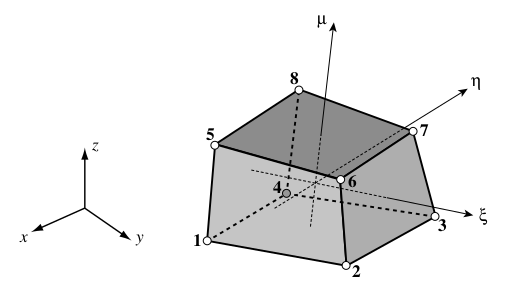
\includegraphics[width=0.90\textwidth]{img/hex8-node-numbers.png}
    \caption{The 8-node hexahedron and the natural coordinates $ \eta $, $ \xi $
    and $ \mu $.}
    \label{fig:hex8-node-numbers-png}
\end{figure}


\subsubsection{Element Definition}

The 8-noded hexahedral element is defined by:

\begin{eqarray}
    \begin{bmatrix}
        1\\
        x\\
        y\\
        z\\
        u_x\\
        u_y\\
        u_z
    \end{bmatrix} &=
    \begin{bmatrix}
        1 & 1 & 1 & 1 & 1 & 1 & 1 & 1\\
        x_1 & x_2 & x_3 & x_4 & x_5 & x_6 & x_7 & x_8\\
        y_1 & y_2 & y_3 & y_4 & y_5 & y_6 & y_7 & y_8\\
        y_1 & y_2 & y_3 & y_4 & y_5 & y_6 & y_7 & y_8\\
        u_{x1} & u_{x2} & u_{x3} & u_{x4} & u_{x5} & u_{x6} & u_{x7} & u_{x8}\\
        u_{y1} & u_{y2} & u_{y3} & u_{y4} & u_{y5} & u_{y6} & u_{y7} & u_{y8}\\
        u_{z1} & u_{z2} & u_{z3} & u_{z4} & u_{z5} & u_{z6} & u_{z7} & u_{z8}
    \end{bmatrix}
    \begin{bmatrix}
        N_1^e\\
        N_2^e\\
        N_3^e\\
        N_4^e\\
        N_5^e\\
        N_6^e\\
        N_7^e\\
        N_8^e
    \end{bmatrix}
\end{eqarray}

The hexahedron corners natural coordinates are:

\begin{table}[ht]
    \centering
    \begin{tabular}{|c c c c|}
        \hline
        node & $\xi$ & $\eta$ & $\mu$\\
        \hline
        1 & -1 & -1 & -1\\
        2 & +1 & -1 & -1\\
        3 & +1 & +1 & -1\\
        4 & -1 & +1 & -1\\
        5 & -1 & -1 & +1\\
        6 & +1 & -1 & +1\\
        7 & +1 & +1 & +1\\
        8 & -1 & +1 & +1\\
        \hline
    \end{tabular}\\
    \caption{Hexahedron corners natural coordinates}
\end{table}

The shape functions are:
\begin{eqarray}
    N_1^e &= \frac{1}{8} \left(1-\xi\right) \left(1-\eta\right) \left(1-\mu\right)\\
    N_2^e &= \frac{1}{8} \left(1+\xi\right) \left(1-\eta\right) \left(1-\mu\right)\\
    N_3^e &= \frac{1}{8} \left(1+\xi\right) \left(1+\eta\right) \left(1-\mu\right)\\
    N_4^e &= \frac{1}{8} \left(1-\xi\right) \left(1+\eta\right) \left(1-\mu\right)\\
    N_5^e &= \frac{1}{8} \left(1-\xi\right) \left(1-\eta\right) \left(1+\mu\right)\\
    N_6^e &= \frac{1}{8} \left(1+\xi\right) \left(1-\eta\right) \left(1+\mu\right)\\
    N_7^e &= \frac{1}{8} \left(1+\xi\right) \left(1+\eta\right) \left(1+\mu\right)\\
    N_8^e &= \frac{1}{8} \left(1-\xi\right) \left(1+\eta\right) \left(1+\mu\right)
\end{eqarray}

\begin{bbox}[0.96]
    The eight formulas can be summarised in a single expression:

    \begin{equation}
        N_i^e = \frac{1}{8}
              \left(1+\xi\xi_i\right)
              \left(1+\eta\eta_i\right)
              \left(1+\mu\mu_i\right)
    \end{equation}

    where $\xi_i$, $\eta_i$ and $\mu_i$ denote the coordinates of the $i$-th node.
\end{bbox}


\subsubsection{Partial Derivatives}
The calculation of the shape functions derivatives with respect to the natural
coordinates:

\begin{eqarray}
    \frac{\partial N_1^e}{\partial\xi} &= -\frac{1}{8} \left(1-\eta\right) \left(1-\mu\right)\\
    \frac{\partial N_2^e}{\partial\xi} &= \phantom{-}\frac{1}{8} \left(1-\eta\right) \left(1-\mu\right)\\
    \frac{\partial N_3^e}{\partial\xi} &= \phantom{-}\frac{1}{8} \left(1+\eta\right) \left(1-\mu\right)\\
    \frac{\partial N_4^e}{\partial\xi} &= -\frac{1}{8} \left(1+\eta\right) \left(1-\mu\right)\\
    \frac{\partial N_5^e}{\partial\xi} &= -\frac{1}{8} \left(1-\eta\right) \left(1+\mu\right)\\
    \frac{\partial N_6^e}{\partial\xi} &= \phantom{-}\frac{1}{8} \left(1-\eta\right) \left(1+\mu\right)\\
    \frac{\partial N_7^e}{\partial\xi} &= \phantom{-}\frac{1}{8} \left(1+\eta\right) \left(1+\mu\right)\\
    \frac{\partial N_8^e}{\partial\xi} &= -\frac{1}{8} \left(1+\eta\right) \left(1+\mu\right)
\end{eqarray}

\begin{eqarray}
    \frac{\partial N_1^e}{\partial\eta} &= -\frac{1}{8} \left(1-\xi\right) \left(1-\mu\right)\\
    \frac{\partial N_2^e}{\partial\eta} &= -\frac{1}{8} \left(1+\xi\right) \left(1-\mu\right)\\
    \frac{\partial N_3^e}{\partial\eta} &= \phantom{-}\frac{1}{8} \left(1+\xi\right) \left(1-\mu\right)\\
    \frac{\partial N_4^e}{\partial\eta} &= \phantom{-}\frac{1}{8} \left(1-\xi\right) \left(1-\mu\right)\\
    \frac{\partial N_5^e}{\partial\eta} &= -\frac{1}{8} \left(1-\xi\right) \left(1+\mu\right)\\
    \frac{\partial N_6^e}{\partial\eta} &= -\frac{1}{8} \left(1+\xi\right) \left(1+\mu\right)\\
    \frac{\partial N_7^e}{\partial\eta} &= \phantom{-}\frac{1}{8} \left(1+\xi\right) \left(1+\mu\right)\\
    \frac{\partial N_8^e}{\partial\eta} &= \phantom{-}\frac{1}{8} \left(1-\xi\right) \left(1+\mu\right)
\end{eqarray}

\begin{eqarray}
    \frac{\partial N_1^e}{\partial\mu} &= -\frac{1}{8} \left(1-\xi\right) \left(1-\eta\right)\\
    \frac{\partial N_2^e}{\partial\mu} &= -\frac{1}{8} \left(1+\xi\right) \left(1-\eta\right)\\
    \frac{\partial N_3^e}{\partial\mu} &= -\frac{1}{8} \left(1+\xi\right) \left(1+\eta\right)\\
    \frac{\partial N_4^e}{\partial\mu} &= -\frac{1}{8} \left(1-\xi\right) \left(1+\eta\right)\\
    \frac{\partial N_5^e}{\partial\mu} &= \phantom{-}\frac{1}{8} \left(1-\xi\right) \left(1-\eta\right)\\
    \frac{\partial N_6^e}{\partial\mu} &= \phantom{-}\frac{1}{8} \left(1+\xi\right) \left(1-\eta\right)\\
    \frac{\partial N_7^e}{\partial\mu} &= \phantom{-}\frac{1}{8} \left(1+\xi\right) \left(1+\eta\right)\\
    \frac{\partial N_8^e}{\partial\mu} &= \phantom{-}\frac{1}{8} \left(1-\xi\right) \left(1+\eta\right)
\end{eqarray}

\begin{bbox}
    \textbf{Note:}

    The partial derivatives can be also written as:

    \begin{eqarray}
        \frac{\partial N_i^e}{\partial \xi} &= \frac{1}{8} \frac{\xi_i}{|\xi_i|}
            \left(1+\eta\eta_i\right) \left(1+\mu\mu_i\right) \\
        \frac{\partial N_i^e}{\partial \eta} &= \frac{1}{8} \frac{\eta_i}{|\eta_i|}
            \left(1+\xi\xi_i\right) \left(1+\mu\mu_i\right) \\
        \frac{\partial N_i^e}{\partial \mu} &= \frac{1}{8} \frac{\mu_i}{|\mu_i|}
            \left(1+\xi\xi_i\right) \left(1+\eta\eta_i\right)
    \end{eqarray}
\end{bbox}



\textbf{The Jacobian:}

The derivatives of the shape functions are given by the usual chain rule formulas:

\begin{eqarray}
    \frac{\partial N_i^e}{\partial x} &=
        \frac{\partial N_i^e}{\partial \xi} \frac{\partial \xi}{\partial x} +
        \frac{\partial N_i^e}{\partial \eta} \frac{\partial \eta}{\partial x} +
        \frac{\partial N_i^e}{\partial \mu} \frac{\partial \mu}{\partial x}\\
    \frac{\partial N_i^e}{\partial y} &=
        \frac{\partial N_i^e}{\partial \xi} \frac{\partial \xi}{\partial y} +
        \frac{\partial N_i^e}{\partial \eta} \frac{\partial \eta}{\partial y} +
        \frac{\partial N_i^e}{\partial \mu} \frac{\partial \mu}{\partial y}\\
    \frac{\partial N_i^e}{\partial z} &=
        \frac{\partial N_i^e}{\partial \xi} \frac{\partial \xi}{\partial z} +
        \frac{\partial N_i^e}{\partial \eta} \frac{\partial \eta}{\partial z} +
        \frac{\partial N_i^e}{\partial \mu} \frac{\partial \mu}{\partial z}
\end{eqarray}

In matrix form:

\begin{eqarray}
    \begin{bmatrix}
        \frac{\partial N_i^e}{\partial x}\\
        \frac{\partial N_i^e}{\partial y}\\
        \frac{\partial N_i^e}{\partial z}
    \end{bmatrix} &=
    \begin{bmatrix}
        \frac{\partial \xi}{\partial x} &
        \frac{\partial \eta}{\partial x} &
        \frac{\partial \mu}{\partial x}\\
        \frac{\partial \xi}{\partial y} &
        \frac{\partial \eta}{\partial y} &
        \frac{\partial \mu}{\partial y}\\
        \frac{\partial \xi}{\partial z} &
        \frac{\partial \eta}{\partial z} &
        \frac{\partial \mu}{\partial z}
    \end{bmatrix}
    \begin{bmatrix}
        \frac{\partial N_i^e}{\partial \xi}\\
        \frac{\partial N_i^e}{\partial \eta}\\
        \frac{\partial N_i^e}{\partial \mu}
    \end{bmatrix}
\end{eqarray}

The $ 3 \times 3 $ matrix above is $ \m{J}^{-1} $, the inverse of:
\begin{eqarray}
    \m{J} = \frac{\partial \left( x, y, z \right)}{\partial \left( \xi, \eta, \mu \right)}
    = \begin{bmatrix}
        \frac{\partial x}{\partial \xi} &
        \frac{\partial y}{\partial \xi} &
        \frac{\partial z}{\partial \xi} \\
        \frac{\partial x}{\partial \eta} &
        \frac{\partial y}{\partial \eta} &
        \frac{\partial z}{\partial \eta} \\
        \frac{\partial x}{\partial \mu} &
        \frac{\partial y}{\partial \mu} &
        \frac{\partial z}{\partial \mu}
    \end{bmatrix}
\end{eqarray}

Matrix $ \m{J} $ is called the \textit{Jacobian matrix} of $ (x, y, z) $
with respect to $ (\xi, \eta, \mu) $. In the finite element literature, matrices
$ \m{J} $ and $ \m{J}^{-1} $ are called simply the \textit{Jacobian} and
\textit{inverse Jacobian}, respectively, although such a short name us sometimes
ambiguous. The notation

\begin{eqarray}
    \m{J} &=
    \frac{\partial \left(x, y, z \right)}{\partial \left(\xi, \eta, \mu \right)}\\
    \m{J}^{-1} &=
    \frac{\partial \left(\xi, \eta, \mu \right)}{\partial \left(x, y, z \right)}
\end{eqarray}

is standard in multivariable calculus and suggests that the Jacobian may be viewed as
a generalisation of the ordinary derivativem to which it reduces for a scalar
function $ \m{x} = x(\xi) $.



\subsubsection{Computing the Jacobian Matrix}
The isoparametric definitioin of hexahedron element geometry is:

\begin{eqarray}
    x &= x_i N_i^e\\
    y &= y_i N_i^e\\
    z &= z_i N_i^e
\end{eqarray}

where the summation convention is understood to apply over $ i = 1, 2, \dots , n $,
in which $ n $ denotes the number of element nodes.

\begin{bbox}
    \textbf{Note:} This for a given hexahedral element gives an $ n \times 3 $ matrix.
\end{bbox}


Differentiating these relations with respect to the hexahedron coordinates we construct
the matrix $ \m{J} $ as follows:

\begin{equation}
    \m{J} =
    \begin{bmatrix}
        x_i \frac{\partial N_i^e}{\partial \xi} &
        y_i \frac{\partial N_i^e}{\partial \xi} &
        z_i \frac{\partial N_i^e}{\partial \xi}\\
        x_i \frac{\partial N_i^e}{\partial \eta} &
        y_i \frac{\partial N_i^e}{\partial \eta} &
        z_i \frac{\partial N_i^e}{\partial \eta}\\
        x_i \frac{\partial N_i^e}{\partial \mu} &
        y_i \frac{\partial N_i^e}{\partial \mu} &
        z_i \frac{\partial N_i^e}{\partial \mu}
    \end{bmatrix}
\end{equation}

or:
\begin{equation}
    \m{J}_i =
    \begin{bmatrix}
        \frac{\partial N_1^e}{\partial \xi} &
        \frac{\partial N_2^e}{\partial \xi} &
        \dots &
        \frac{\partial N_n^e}{\partial \xi}\\
        \frac{\partial N_1^e}{\partial \eta} &
        \frac{\partial N_2^e}{\partial \eta} &
        \dots &
        \frac{\partial N_n^e}{\partial \eta}\\
        \frac{\partial N_1^e}{\partial \mu} &
        \frac{\partial N_2^e}{\partial \mu} &
        \dots &
        \frac{\partial N_n^e}{\partial \mu}
    \end{bmatrix}
    \begin{bmatrix}
        x_1 & y_1 & z_1 \\
        x_2 & y_2 & z_2 \\
        \vdots & \vdots & \vdots \\
        x_n & y_n & z_n
    \end{bmatrix}
\end{equation}


Given a point of hexahedron coordinates $ ( \xi, \eta, \mu ) $ the Jacobian $ \m{J} $
can be easilly formed using the above formula, and numerically inverted to form
$ \m{J}^{-1} $.


\subsubsection{The Strain-Displacement Matrix}

Having obtained the shape function derivatives, the matrix $ \m{B} $ for hexahedron
element displays the usual structure for 3D elements:

\begin{equation}
    \m{B} = \m{D}\m{\Phi} =
    \begin{bmatrix}
        \frac{\partial}{\partial x} & 0 & 0 \\
        0 & \frac{\partial}{\partial y} & 0 \\
        0 & 0 & \frac{\partial}{\partial z} \\
        \frac{\partial}{\partial y} & \frac{\partial}{\partial x} & 0 \\
        0 & \frac{\partial}{\partial z} & \frac{\partial}{\partial y} \\
        \frac{\partial}{\partial z} & 0 & \frac{\partial}{\partial x}
    \end{bmatrix}
    \begin{bmatrix}
        \m{q} & \m{0} & \m{0} \\
        \m{0} & \m{q} & \m{0} \\
        \m{0} & \m{0} & \m{q}
    \end{bmatrix} =
    \begin{bmatrix}
        \m{q}_x & \m{0} & \m{0} \\
        \m{0} & \m{q}_y & \m{0} \\
        \m{0} & \m{0} & \m{q}_z \\
        \m{q}_y & \m{q}_x & \m{0} \\
        \m{0} & \m{q}_z & \m{q}_y \\
        \m{q}_z & \m{0} & \m{q}_x
    \end{bmatrix}
\end{equation}

where:
\begin{eqarray}
    \m{q} &= \begin{bmatrix} N_1^e & \dots & N_n^e \end{bmatrix}\\
    \m{q}_x &= \begin{bmatrix} \frac{\partial N_1^e}{\partial x} & \dots & \frac{\partial N_n^e}{\partial x} \end{bmatrix}\\
    \m{q}_y &= \begin{bmatrix} \frac{\partial N_1^e}{\partial y} & \dots & \frac{\partial N_n^e}{\partial y} \end{bmatrix}\\
    \m{q}_z &= \begin{bmatrix} \frac{\partial N_1^e}{\partial z} & \dots & \frac{\partial N_n^e}{\partial z} \end{bmatrix}
\end{eqarray}

are row vectors of length $ n $, $ n $ being the number of nodes in the element.



\subsubsection{Stiffness Matrix Evaluation}

The element stiffness Matrix is given by:

\begin{equation}
    \m{K}^e = \int_{V^e} \m{B}^T \m{E} \m{B} dV^e
\end{equation}

As in two-dimensional case, this is replaced by a numerical integration formula which
now involves a triple loop over conventional Gauss quadrature rules. Assuming that
the stress-strain matrix $ \m{E} $ is constant over the element,

\begin{equation}
    \m{K}^e = \sum_{i=1}^{p_1} \sum_{j=1}^{p_2} \sum_{k=1}^{p_3}
    w_i w_j w_k \m{B}_{ijk}^T \m{E} \m{B}_{ijk} \m{J}_{ijk}
\end{equation}

Here $ p_1 $, $ p_2 $ and $ p_3 $ are the number of Gauss points in the $ \xi $,
$ \eta $ and $ \mu $ direction, respectively, while $ \m{B}_{ijk} $
and $ \m{J}_{ijk} $ are abbreviations for:

\begin{eqarray}
    \m{B}_{ijk} &= \m{B} \left(\xi_i, \eta_i, \mu_i\right) \\
    \m{J}_{ijk} &= det \m{J} \left(\xi_i, \eta_i, \mu_i\right)
\end{eqarray}

Usually the number of integration points is taken the same in all directions:
$ p = p_1 = p_2 = p_3 $. The total number of Gauss points is thus $ p^3 $.
Each point adds at most 6 to the stiffness matrix rank. The minimum rank-sufficient
rules for the 8-node and 20-node hexahedra are $ p = 2 $ and $ p = 3 $, respectively.


\subsection{Python implementation}

\begin{python}
#!/usr/bin/python3

import numpy as np
np.set_printoptions(precision=2) # , suppress=True)

def hex8_stiffness_mass_load(coors: np.ndarray,
                             E: float,
                             nu: float,
                             rho: float,
                             fx: float = 0.,
                             fy: float = 0.,
                             fz: float = 0.):
    """
    In:
        coors - 8 x 3 coordinate matrix
                [[x1,y1,z1], ... , [xn,yn,zn]
        E     - Youngs's Modulus
        nu    - Poisson's Constant
        rho   - Density
        fx    - Volumetric Load in x direction
        fy    - Volumetric Load in y direction
        fz    - Volumetric Load in z direction
    """
    domain = np.array([[-1., -1., -1.],
                       [1., -1., -1.],
                       [1., 1., -1.],
                       [-1., 1., -1.],
                       [-1., -1., 1.],
                       [1., -1., 1.],
                       [1., 1., 1.],
                       [-1., 1., 1.]], dtype=float)
    print('Domain: {0}\n{1}'.format(domain.shape, domain))

    # gaussian interpolation
    gauss_points = 3
    g_points, g_weights = np.polynomial.legendre.leggauss(gauss_points)
    integration_points = []
    interpolation_weights = []
    for i, xi in enumerate(g_points):
        for j, eta in enumerate(g_points):
            for k, mu in enumerate(g_points):
                integration_points.append([xi, eta, mu])
                interpolation_weights.append(g_weights[i] *
                                             g_weights[j] *
                                             g_weights[k])
    integration_points = np.array(integration_points, dtype=float)
    interpolation_weights = np.array(interpolation_weights, dtype=float)
    print('Gauss Integration '
          '{0}:\n{1}\nWeights:\n{2}'.format(gauss_points,
                                            integration_points,
                                            interpolation_weights))

    full_domain = np.vstack((domain, integration_points))

    # Shape Functions in Natural Coordinates
    xi = integration_points.T[0]
    eta = integration_points.T[1]
    mu = integration_points.T[2]
    psi = np.zeros((8, integration_points.shape[0]), dtype=float)
    for i in range(8):
        psi[i] = 1/8 * (1 + xi * domain[i, 0]) *
                       (1 + eta * domain[i, 1]) *
                       (1 + mu * domain[i, 2])
    psi = psi.T
    print('Shape Functions: {0}\n{1}'.format(psi.shape, psi))

    # Shape Functions in Global Coordinates
    psi_g = psi @ coors
    print('Shape Functions in '
          'Global Coordinates: {0}\n{1}'.format(psi_g.shape, psi_g))

    # Shape Functions Derivatives in Natural Coordinates
    dpsi = 1 / 8 * np.array([[(eta - 1.0) * (1.0 - mu),# 1
                              (xi - 1) * (1 - mu),
                             -(1 - xi) * (1 - eta)],
                             [(1 - eta) * (1 - mu),    # 2
                              (-1 - xi) * (1 - mu),
                             -(1 + xi) * (1 - eta)],
                             [(1 + eta) * (1 - mu),    # 3
                              (1 + xi) * (1 - mu),
                             -(1 + xi) * (1 + eta)],
                             [(-1.0 - eta) * (1 - mu), # 4
                              (1 - xi) * (1 - mu),
                             -(1 - xi) * (1 + eta)],
                             [(1 - eta) * (-1 - mu),   # 5
                             -(1 - xi) * (1 + mu),
                              (1 - xi) * (1 - eta)],
                             [(1 - eta) * (1 + mu),    # 6
                             -(1 + xi) * (1 + mu),
                              (1 + xi) * (1 - eta)],
                             [(1 + eta) * (1 + mu),    # 7
                              (1 + xi) * (1 + mu),
                              (1 + xi) * (1 + eta)],
                             [-(1 + eta) * (1 + mu),   # 8
                              (1 - xi) * (1 + mu),
                              (1 - xi) * (1 + eta)]])
    dpsi = dpsi.T
    print('Shape Functions Derivatives: '
          '{0}\n{1}'.format(dpsi.shape, dpsi))

    # Jacobian Matrix
    jacobi = dpsi @ coors
    print('Jacobian Matrix: {0}\n{1}'.format(jacobi.shape, jacobi))

    # Jacobian Determinants
    d_jacobi = np.linalg.det(jacobi)
    print('Determinant of Jacobian: '
          '{0}\n{1}'.format(d_jacobi.shape, d_jacobi))

    # Inverse Jacobian
    i_jacobi = np.linalg.inv(jacobi)
    print('Inverse Jacobian Matrix: '
          '{0}\n{1}'.format(i_jacobi.shape, i_jacobi))

    # Shape Function Derivatives in Global Coordinates
    dpsi_g = i_jacobi @ dpsi
    print('Shape Function Derivatives in Global Coordinates: '
          '{0}\n{1}'.format(dpsi_g.shape, dpsi_g))

    # Material Stiffness Matrix
    C = E / ((1.0 + nu) * (1.0 - 2.0 * nu)) *
        np.array([[1.0 - nu, nu, nu, 0.0, 0.0, 0.0],
                  [nu, 1.0 - nu, nu, 0.0, 0.0, 0.0],
                  [nu, nu, 1.0 - nu, 0.0, 0.0, 0.0],
                  [0.0, 0.0, 0.0, (1.0 - 2.0 * nu) / 2.0, 0.0, 0.0],
                  [0.0, 0.0, 0.0, 0.0, (1.0 - 2.0 * nu) / 2.0, 0.0],
                  [0.0, 0.0, 0.0, 0.0, 0.0, (1.0 - 2.0 * nu) / 2.0]],
                  dtype=float)
    print('Material Stiffness Matrix: {0}\n{1}'.format(C.shape, C))

    # Create Element Stiffness and Mass Matrix
    Ke = np.zeros((domain.size, domain.size), dtype=float)
    Me = np.zeros((domain.size, domain.size), dtype=float)
    Fe = np.zeros((domain.size, 1), dtype=float)
    # o = np.zeros(domain.shape[0], dtype=float)

    # iterate over Gauss points of domain, * means unpack values
    for i in range(integration_points.shape[0]):
        # this is smart but arranges dofs by component, not by node
        # component-wise dof ordering (x1, .. , y1, .. y4, z1, .. , z4)
        # B = np.array([
        #   [*dpsi_g[i, 0, :], *o, *o],
        #   [*o, *dpsi_g[i, 1, :], *o],
        #   [*o, *o, *dpsi_g[i, 2, :]],
        #   [*dpsi_g[i, 2, :], *o, *dpsi_g[i, 0, :]],
        #   [*o, *dpsi_g[i, 2, :], *dpsi_g[i, 1, :]],
        #   [*dpsi_g[i, 1, :], *dpsi_g[i, 0, :], *o]], dtype=float)

        # dofs ordered by node
        # node wise dof ordering (x1, y1, z1, .. , x4, y4, z4)
        dpx = dpsi_g[i,0,:]
        dpy = dpsi_g[i,1,:]
        dpz = dpsi_g[i,2,:]
        # B = np.array(
        #     [[dpx[0],0,0,dpx[1],0,0,dpx[2],0,0,dpx[3],0,0,dpx[4],0,0,dpx[5],0,0,dpx[6],0,0,dpx[7],0,0],
        #      [0,dpy[0],0,0,dpy[1],0,0,dpy[2],0,0,dpy[3],0,0,dpy[4],0,0,dpy[5],0,0,dpy[6],0,0,dpy[7],0],
        #      [0,0,dpz[0],0,0,dpz[1],0,0,dpz[2],0,0,dpz[3],0,0,dpz[4],0,0,dpz[5],0,0,dpz[6],0,0,dpz[7]],
        #      [dpy[0],dpx[0],0,dpy[1],dpx[1],0,dpy[2],dpx[2],0,dpy[3],dpx[3],0,dpy[4],dpx[4],0,dpy[5],dpx[5],0,dpy[6],dpx[6],0,dpy[7],dpx[7],0],
        #      [0,dpz[0],dpy[0],0,dpz[1],dpy[1],0,dpz[2],dpy[2],0,dpz[3],dpy[3],0,dpz[4],dpy[4],0,dpz[5],dpy[5],0,dpz[6],dpy[6],0,dpz[7],dpy[7]],
        #      [dpz[0],0,dpx[0],dpz[1],0,dpx[1],dpz[2],0,dpx[2],dpz[3],0,dpx[3],dpz[4],0,dpx[4],dpz[5],0,dpx[5],dpz[6],0,dpx[6],dpz[7],0,dpx[7]]],
        #      dtype=_FLOAT)
        B = np.array([np.column_stack((dpx,   o,   o)).flatten(),
                      np.column_stack((  o, dpy,   o)).flatten(),
                      np.column_stack((  o,   o, dpz)).flatten(),
                      np.column_stack((dpy, dpx,   o)).flatten(),
                      np.column_stack((  o, dpz, dpy)).flatten(),
                      np.column_stack((dpz,   o, dpx)).flatten()], dtype=float)

        # this is smart but arranges dofs by component, not by node
        # component-wise dof ordering (x1, .. , y1, .. y4, z1, .. , z4)
        # N = np.array([
        #   [*psi[i], *o, *o],
        #   [*o, *psi[i], *o],
        #   [*o, *o, *psi[i]]],
        #   dtype=float)

        # node wise dof ordering (x1, y1, z1, .. , x4, y4, z4)
        # N = np.array([[p[0],0,0,p[1],0,0,p[2],0,0,p[3],0,0,p[4],0,0,p[5],0,0,p[6],0,0,p[7],0,0],
        #               [0,p[0],0,0,p[1],0,0,p[2],0,0,p[3],0,0,p[4],0,0,p[5],0,0,p[6],0,0,p[7],0],
        #               [0,0,p[0],0,0,p[1],0,0,p[2],0,0,p[3],0,0,p[4],0,0,p[5],0,0,p[6],0,0,p[7]]],
        #               dtype=_FLOAT)
        N = np.array([np.column_stack((p, o, o)).flatten(),
                      np.column_stack((o, p, o)).flatten(),
                      np.column_stack((p, o, o)).flatten()], dtype=float)

        F = np.array([[fx], [fy], [fz]], dtype=float)

        Ke += (B.T @ C @ B) * d_jacobi[i] * interpolation_weights[i]
        Me += rho * (N.T @ N) * d_jacobi[i] * interpolation_weights[i]
        Fe += (N.T @ F) * d_jacobi[i] * interpolation_weights[i]

    print('Element Stiffness Matrix: {0}\n{1}'.format(Ke.shape, Ke))
    print('Element Mass Matrix: {0}\n{1}'.format(Me.shape, Me))
    print('Element Volume Force Vector: {0}\n{1}'.format(Fe.shape, Fe))
\end{python}

And to get stresses:
\begin{python}
#!/usr/bin/python3

import numpy as np
np.set_printoptions(precision=2) # , suppress=True)

def hex8_stresses(coors: np.ndarray,
                  disp: np.ndarray,
                  E: float,
                  nu: float):
    """
    In:
        coors - 8 x 3 coordinate matrix
                [[x1,y1,z1], ... , [xn,yn,zn]
        disp  - 8 x 3 coordinate matrix
                [[u1,v1,w1], ... , [un,vn,wn]
        E     - Youngs's Modulus
        nu    - Poisson's Constant
    """
    domain = np.array([[-1., -1., -1.],
                       [1., -1., -1.],
                       [1., 1., -1.],
                       [-1., 1., -1.],
                       [-1., -1., 1.],
                       [1., -1., 1.],
                       [1., 1., 1.],
                       [-1., 1., 1.]], dtype=float)
    print('Domain: {0}\n{1}'.format(domain.shape, domain))

    # gaussian interpolation
    gauss_points = 3
    g_points, g_weights = np.polynomial.legendre.leggauss(gauss_points)
    integration_points = []
    interpolation_weights = []
    for i, xi in enumerate(g_points):
        for j, eta in enumerate(g_points):
            for k, mu in enumerate(g_points):
                integration_points.append([xi, eta, mu])
                interpolation_weights.append(g_weights[i] *
                                             g_weights[j] *
                                             g_weights[k])
    integration_points = np.array(integration_points, dtype=float)
    interpolation_weights = np.array(interpolation_weights, dtype=float)
    print('Gauss Integration '
          '{0}:\n{1}\nWeights:\n{2}'.format(gauss_points,
                                            integration_points,
                                            interpolation_weights))

    full_domain = np.vstack((domain, integration_points))

    # Shape Functions in Natural Coordinates
    xi = integration_points.T[0]
    eta = integration_points.T[1]
    mu = integration_points.T[2]
    psi = np.zeros((8, integration_points.shape[0]), dtype=float)
    for i in range(8):
        psi[i] = 1/8 * (1 + xi * domain[i, 0]) *
                       (1 + eta * domain[i, 1]) *
                       (1 + mu * domain[i, 2])
    psi = psi.T
    print('Shape Functions: {0}\n{1}'.format(psi.shape, psi))

    # Shape Functions in Global Coordinates
    psi_g = psi @ coors
    print('Shape Functions in '
          'Global Coordinates: {0}\n{1}'.format(psi_g.shape, psi_g))

    # Shape Functions Derivatives in Natural Coordinates
    dpsi = 1 / 8 * np.array([[(eta - 1.0) * (1.0 - mu),# 1
                              (xi - 1) * (1 - mu),
                             -(1 - xi) * (1 - eta)],
                             [(1 - eta) * (1 - mu),    # 2
                              (-1 - xi) * (1 - mu),
                             -(1 + xi) * (1 - eta)],
                             [(1 + eta) * (1 - mu),    # 3
                              (1 + xi) * (1 - mu),
                             -(1 + xi) * (1 + eta)],
                             [(-1.0 - eta) * (1 - mu), # 4
                              (1 - xi) * (1 - mu),
                             -(1 - xi) * (1 + eta)],
                             [(1 - eta) * (-1 - mu),   # 5
                             -(1 - xi) * (1 + mu),
                              (1 - xi) * (1 - eta)],
                             [(1 - eta) * (1 + mu),    # 6
                             -(1 + xi) * (1 + mu),
                              (1 + xi) * (1 - eta)],
                             [(1 + eta) * (1 + mu),    # 7
                              (1 + xi) * (1 + mu),
                              (1 + xi) * (1 + eta)],
                             [-(1 + eta) * (1 + mu),   # 8
                              (1 - xi) * (1 + mu),
                              (1 - xi) * (1 + eta)]])
    dpsi = dpsi.T
    print('Shape Functions Derivatives: '
          '{0}\n{1}'.format(dpsi.shape, dpsi))

    # Jacobian Matrix
    jacobi = dpsi @ coors
    print('Jacobian Matrix: {0}\n{1}'.format(jacobi.shape, jacobi))

    # Jacobian Determinants
    d_jacobi = np.linalg.det(jacobi)
    print('Determinant of Jacobian: '
          '{0}\n{1}'.format(d_jacobi.shape, d_jacobi))

    # Inverse Jacobian
    i_jacobi = np.linalg.inv(jacobi)
    print('Inverse Jacobian Matrix: '
          '{0}\n{1}'.format(i_jacobi.shape, i_jacobi))

    # Shape Function Derivatives in Global Coordinates
    dpsi_g = i_jacobi @ dpsi
    print('Shape Function Derivatives in Global Coordinates: '
          '{0}\n{1}'.format(dpsi_g.shape, dpsi_g))

    # Material Stiffness Matrix
    C = E / ((1.0 + nu) * (1.0 - 2.0 * nu)) *
        np.array([[1.0 - nu, nu, nu, 0.0, 0.0, 0.0],
                  [nu, 1.0 - nu, nu, 0.0, 0.0, 0.0],
                  [nu, nu, 1.0 - nu, 0.0, 0.0, 0.0],
                  [0.0, 0.0, 0.0, (1.0 - 2.0 * nu) / 2.0, 0.0, 0.0],
                  [0.0, 0.0, 0.0, 0.0, (1.0 - 2.0 * nu) / 2.0, 0.0],
                  [0.0, 0.0, 0.0, 0.0, 0.0, (1.0 - 2.0 * nu) / 2.0]],
                  dtype=float)
    print('Material Stiffness Matrix: {0}\n{1}'.format(C.shape, C))

    du = disp.T @ np.transpose(dpsi_g, axes=[0, 2, 1])

    exx = du[:, 0, 0]
    eyy = du[:, 1, 1]
    ezz = du[:, 2, 2]
    exy = du[:, 0, 1] + du[:, 1, 0]
    eyz = du[:, 1, 2] + du[:, 2, 1]
    exz = du[:, 0, 2] + du[:, 2, 0]
    epsilons = np.array([exx, eyy, ezz, exy, eyz, exz])

    sigmas = (C @ epsilons).T
    epsilons = epsilons.T
    print('Element Strains: {0}\n{1}'.format(epsilons.shape, epsilons))
    print('Element Stresses: {0}\n{1}'.format(stresses.shape, stresses))
\end{python}




\newpage
\section{TET4 Element}

\subsection{Element Formulation}
For a linear tetrahedron no numerical integration is needed (there can be only
one integration point, shape functions derivatives are equal to 1).

The linear tetrahedron is not often used for stress analysis because of its poor
performance. Its main value in structural and solid mechanics is educational:
it serves as a vehicle to introduce the basic steps of formulation of 3D solid elements,
particularly with regards to the use of natural coordinate systems and node numbering
conventions. It should be noted that 3D visualisation is notoriously more difficult
than 2D, so it is needed to procede more slowly here.

\begin{figure}[ht]
    \centering
    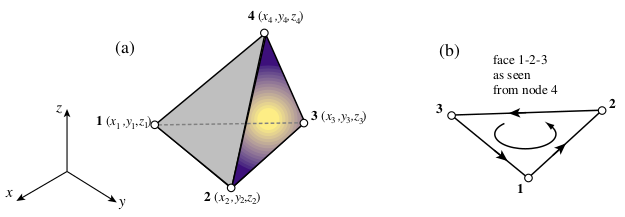
\includegraphics[width=0.90\textwidth]{img/linear_tetrahedron.png}
    \caption{(a)The linear tetrahedron element TET4, (b) Node numbering convention.}
    \label{fig:linear-tetrahedron-png}
\end{figure}


\subsubsection{Tetrahedron Geometry}

The tetrahedron geometry is fully defined by giving the location of the four
corner nodes with respect to Right-Hand Coordinate Sysetm notation $ (x, y, z) $:




\subsection{Python Implementation}
\begin{python}
#!/usr/bin/python3

import numpy as np
np.set_printoptions(precision=2) # , suppress=True)

def tet4_stiffness_mass_load(coors: np.ndarray,
                             E: float,
                             nu: float,
                             rho: float,
                             fx: float = 0.,
                             fy: float = 0.,
                             fz: float = 0.,
                             gauss_points = 4):
    domain = np.array([[1., 0., 0., 0.],
                       [0., 1., 0., 0.],
                       [0., 0., 1., 0.],
                       [0., 0., 0., 1.]], dtype=float)
    print('Domain: {0}\n{1}'.format(domain.shape, domain))

    # gaussian interpolation
    integration_points = None
    integration_weights = None
    if gauss_points == 1:
        integration_points = np.array([1/4, 1/4, 1/4, 1/4],
                                      dtype=float).reshape(1, 4)
        integration_weights = np.array([1 * 1 * 1 * 1],
                                       dtype=float) * 1/6

    elif gauss_points == 4:
        a = 0.58541020
        b = 0.13819660
        integration_points = np.array([[a, b, b, b],
                                       [b, a, b, b],
                                       [b, b, a, b],
                                       [b, b, b, a]], dtype=float)
        integration_weights = np.array([1/4, 1/4, 1/4, 1/4],
                                       dtype=float) * 1/6

    elif gauss_points == 5:
        integration_points = np.array([[1/4, 1/4, 1/4, 1/4],
                                       [1/2, 1/6, 1/6, 1/6],
                                       [1/6, 1/2, 1/6, 1/6],
                                       [1/6, 1/6, 1/2, 1/6],
                                       [1/6, 1/6, 1/6, 1/2]], dtype=float)
        integration_weights = np.array([-4/5, 9/20, 9/20, 9/20, 9/20],
                                       dtype=float) * 1/6

    print('Gauss Integration '
          '{0}:\n{1}\nWeights:\n{2}'.format(gauss_points,
                                            integration_points,
                                            integration_weights))

    full_domain = np.vstack((domain, integration_points))

    # Shape Functions in Natural Coordinates
    xi = integration_points.T[0]
    eta = integration_points.T[1]
    mu = integration_points.T[2]
    # zeta is not used to enforce
    # (1 - xi - eta - mu - zeta) = 0
    # zeta = integration_points.T[3]
    psi = np.zeros((4, integration_points.shape[0]), dtype=float)
    # another way of writing that psi = [xi, eta, mu, zeta]
    # for i in range(4):
    #     psi[i] = (1 + xi * domain[i, 0]) * (1 + eta * domain[i, 1]) * (1 + mu * domain[i, 2]) * (1 + zeta * domain[i, 3])
    psi[0] = xi
    psi[1] = eta
    psi[2] = mu
    psi[3] = 1 - xi - eta - mu  # = zeta
    psi = psi.T
    print('Shape Functions: {0}\n{1}'.format(psi.shape, psi))

    # Shape Functions in Global Coordinates
    psi_g = psi @ coors
    print('Shape Functions in Global Coordinates: '
          '{0}\n{1}'.format(psi_g.shape, psi_g))

    # Shape Functions Derivatives in Natural Coordinates
    dpsi = np.zeros((integration_points.shape[0], 4, 3), dtype=float)
    dpsi[:,0,0] = 1
    dpsi[:,1,1] = 1
    dpsi[:,2,2] = 1
    dpsi[:,3,:] = -1
    dpsi = dpsi.transpose((0, 2, 1))
    print('Shape Functions Derivatives: '
          '{0}\n{1}'.format(dpsi.shape, dpsi))

    # Jacobian Matrix
    jacobi = dpsi @ coors
    print('Jacobian Matrix: {0}\n{1}'.format(jacobi.shape, jacobi))

    # Jacobian Determinants
    d_jacobi = np.linalg.det(jacobi)
    print('Determinant of Jacobian: '
          '{0}\n{1}'.format(d_jacobi.shape, d_jacobi))

    # Inverse Jacobian
    i_jacobi = np.linalg.inv(jacobi)
    print('Inverse Jacobian Matrix: '
          '{0}\n{1}'.format(i_jacobi.shape, i_jacobi))

    # Shape Function Derivatives in Global Coordinates
    dpsi_g = i_jacobi @ dpsi
    print('Shape Function Derivatives in Global Coordinates: '
          '{0}\n{1}'.format(dpsi_g.shape, dpsi_g))

    # Material Stiffness Matrix
    C = E / ((1.0 + nu) * (1.0 - 2.0 * nu)) *
        np.array([[1.0 - nu, nu, nu, 0.0, 0.0, 0.0],
                  [nu, 1.0 - nu, nu, 0.0, 0.0, 0.0],
                  [nu, nu, 1.0 - nu, 0.0, 0.0, 0.0],
                  [0.0, 0.0, 0.0, (1.0 - 2.0 * nu) / 2.0, 0.0, 0.0],
                  [0.0, 0.0, 0.0, 0.0, (1.0 - 2.0 * nu) / 2.0, 0.0],
                  [0.0, 0.0, 0.0, 0.0, 0.0, (1.0 - 2.0 * nu) / 2.0]],
                  dtype=float)
    print('Material Stiffness Matrix: {0}\n{1}'.format(C.shape, C))

    # Create Element Stiffness and Mass Matrix
    Ke = np.zeros((domain.shape[0] * 3, domain.shape[0] * 3), dtype=float)
    Me = np.zeros((domain.shape[0] * 3, domain.shape[0] * 3), dtype=float)
    Fe = np.zeros((domain.shape[0] * 3, 1), dtype=float)
    o = np.zeros(domain.shape[0], dtype=float)

    # iterate over Gauss points of domain, * means unpack values
    for i in range(integration_points.shape[0]):
        # component-wise dof ordering (x1, .. , y1, .. y4, z1, .. , z4)
        # B = np.array([[*dpsi_g[i, 0, :], *o, *o],
        #               [*o, *dpsi_g[i, 1, :], *o],
        #               [*o, *o, *dpsi_g[i, 2, :]],
        #               [*dpsi_g[i, 2, :], *o, *dpsi_g[i, 0, :]],
        #               [*o, *dpsi_g[i, 2, :], *dpsi_g[i, 1, :]],
        #               [*dpsi_g[i, 1, :], *dpsi_g[i, 0, :], *o]],
        #               dtype=float)

        # node wise dof ordering (x1, y1, z1, .. , x4, y4, z4)
        dpx = dpsi_g[i,0,:]
        dpy = dpsi_g[i,1,:]
        dpz = dpsi_g[i,2,:]
        B = np.array(
            [[dpx[0],0,0,dpx[1],0,0,dpx[2],0,0,dpx[3],0,0],
             [0,dpy[0],0,0,dpy[1],0,0,dpy[2],0,0,dpy[3],0],
             [0,0,dpz[0],0,0,dpz[1],0,0,dpz[2],0,0,dpz[3]],
             [dpy[0],dpx[0],0,dpy[1],dpx[1],0,dpy[2],dpx[2],0,dpy[3],dpx[3],0],
             [0,dpz[0],dpy[0],0,dpz[1],dpy[1],0,dpz[2],dpy[2],0,dpz[3],dpy[3]],
             [dpz[0],0,dpx[0],dpz[1],0,dpx[1],dpz[2],0,dpx[2],dpz[3],0,dpx[3]],
             dtype=float)

        # component-wise dof ordering (x1, .. , y1, .. y4, z1, .. , z4)
        # N = np.array([[*psi[i], *o, *o],
        #               [*o, *psi[i], *o],
        #               [*o, *o, *psi[i]]], dtype=float)

        # node wise dof ordering (x1, y1, z1, .. , x4, y4, z4)
        N = np.array([[psi[i,0],0,0,psi[i,1],0,0,psi[i,2],0,0,psi[i,3],0,0],
                      [0,psi[i,0],0,0,psi[i,1],0,0,psi[i,2],0,0,psi[i,3],0],
                      [0,0,psi[i,0],0,0,psi[i,1],0,0,psi[i,2],0,0,psi[i,3]],
                      dtype=float)

        F = np.array([[fx], [fy], [fz]], dtype=float)

        print((B.T @ C @ B).shape)
        print(Ke.shape)
        Ke += (B.T @ C @ B) * d_jacobi[i] * integration_weights[i]
        Me += rho * (N.T @ N) * d_jacobi[i] * integration_weights[i]
        Fe += (N.T @ F) * d_jacobi[i] * integration_weights[i]

    print('Element Stiffness Matrix: {0}\n{1}'.format(Ke.shape, Ke))
    print('Element Mass Matrix: {0}\n{1}'.format(Me.shape, Me))
    print('Element Volume Force Vector: {0}\n{1}'.format(Fe.shape, Fe))
\end{python}


And to get stresses:
\begin{python}
#!/usr/bin/python3

import numpy as np
np.set_printoptions(precision=2) # , suppress=True)

def tet4_stresses(coors: np.ndarray,
                  disp: np.ndarray,
                  E: float,
                  nu: float):
    """
    In:
        coors - 4 x 3 coordinate matrix
                [[x1,y1,z1], ... , [xn,yn,zn]
        disp  - 4 x 3 coordinate matrix
                [[u1,v1,w1], ... , [un,vn,wn]
        E     - Youngs's Modulus
        nu    - Poisson's Constant
    """
    domain = np.array([[1., 0., 0., 0.],
                       [0., 1., 0., 0.],
                       [0., 0., 1., 0.],
                       [0., 0., 0., 1.]], dtype=float)
    print('Domain: {0}\n{1}'.format(domain.shape, domain))

    # gaussian interpolation
    integration_points = None
    integration_weights = None
    if gauss_points == 1:
        integration_points = np.array([1/4, 1/4, 1/4, 1/4],
                                      dtype=float).reshape(1, 4)
        integration_weights = np.array([1 * 1 * 1 * 1],
                                       dtype=float) * 1/6

    elif gauss_points == 4:
        a = 0.58541020
        b = 0.13819660
        integration_points = np.array([[a, b, b, b],
                                       [b, a, b, b],
                                       [b, b, a, b],
                                       [b, b, b, a]], dtype=float)
        integration_weights = np.array([1/4, 1/4, 1/4, 1/4],
                                       dtype=float) * 1/6

    elif gauss_points == 5:
        integration_points = np.array([[1/4, 1/4, 1/4, 1/4],
                                       [1/2, 1/6, 1/6, 1/6],
                                       [1/6, 1/2, 1/6, 1/6],
                                       [1/6, 1/6, 1/2, 1/6],
                                       [1/6, 1/6, 1/6, 1/2]], dtype=float)
        integration_weights = np.array([-4/5, 9/20, 9/20, 9/20, 9/20],
                                       dtype=float) * 1/6

    print('Gauss Integration '
          '{0}:\n{1}\nWeights:\n{2}'.format(gauss_points,
                                            integration_points,
                                            integration_weights))

    full_domain = np.vstack((domain, integration_points))

    # Shape Functions in Natural Coordinates
    xi = integration_points.T[0]
    eta = integration_points.T[1]
    mu = integration_points.T[2]
    # zeta is not used to enforce
    # (1 - xi - eta - mu - zeta) = 0
    # zeta = integration_points.T[3]
    psi = np.zeros((4, integration_points.shape[0]), dtype=float)
    # another way of writing that psi = [xi, eta, mu, zeta]
    # for i in range(4):
    #     psi[i] = (1 + xi * domain[i, 0]) * (1 + eta * domain[i, 1]) * (1 + mu * domain[i, 2]) * (1 + zeta * domain[i, 3])
    psi[0] = xi
    psi[1] = eta
    psi[2] = mu
    psi[3] = 1 - xi - eta - mu  # = zeta
    psi = psi.T
    print('Shape Functions: {0}\n{1}'.format(psi.shape, psi))

    # Shape Functions in Global Coordinates
    psi_g = psi @ coors
    print('Shape Functions in Global Coordinates: '
          '{0}\n{1}'.format(psi_g.shape, psi_g))

    # Shape Functions Derivatives in Natural Coordinates
    dpsi = np.zeros((integration_points.shape[0], 4, 3), dtype=float)
    dpsi[:,0,0] = 1
    dpsi[:,1,1] = 1
    dpsi[:,2,2] = 1
    dpsi[:,3,:] = -1
    dpsi = dpsi.transpose((0, 2, 1))
    print('Shape Functions Derivatives: '
          '{0}\n{1}'.format(dpsi.shape, dpsi))

    # Jacobian Matrix
    jacobi = dpsi @ coors
    print('Jacobian Matrix: {0}\n{1}'.format(jacobi.shape, jacobi))

    # Jacobian Determinants
    d_jacobi = np.linalg.det(jacobi)
    print('Determinant of Jacobian: '
          '{0}\n{1}'.format(d_jacobi.shape, d_jacobi))

    # Inverse Jacobian
    i_jacobi = np.linalg.inv(jacobi)
    print('Inverse Jacobian Matrix: '
          '{0}\n{1}'.format(i_jacobi.shape, i_jacobi))

    # Shape Function Derivatives in Global Coordinates
    dpsi_g = i_jacobi @ dpsi
    print('Shape Function Derivatives in Global Coordinates: '
          '{0}\n{1}'.format(dpsi_g.shape, dpsi_g))

    # Material Stiffness Matrix
    C = E / ((1.0 + nu) * (1.0 - 2.0 * nu)) *
        np.array([[1.0 - nu, nu, nu, 0.0, 0.0, 0.0],
                  [nu, 1.0 - nu, nu, 0.0, 0.0, 0.0],
                  [nu, nu, 1.0 - nu, 0.0, 0.0, 0.0],
                  [0.0, 0.0, 0.0, (1.0 - 2.0 * nu) / 2.0, 0.0, 0.0],
                  [0.0, 0.0, 0.0, 0.0, (1.0 - 2.0 * nu) / 2.0, 0.0],
                  [0.0, 0.0, 0.0, 0.0, 0.0, (1.0 - 2.0 * nu) / 2.0]],
                  dtype=float)
    print('Material Stiffness Matrix: {0}\n{1}'.format(C.shape, C))
    du = disp.T @ np.transpose(dpsi_g, axes=[0, 2, 1])

    exx = du[:, 0, 0]
    eyy = du[:, 1, 1]
    ezz = du[:, 2, 2]
    exy = du[:, 0, 1] + du[:, 1, 0]
    eyz = du[:, 1, 2] + du[:, 2, 1]
    exz = du[:, 0, 2] + du[:, 2, 0]
    epsilons = np.array([exx, eyy, ezz, exy, eyz, exz])

    sigmas = (C @ epsilons).T
    epsilons = epsilons.T
    print('Element Strains: {0}\n{1}'.format(epsilons.shape, epsilons))
    print('Element Stresses: {0}\n{1}'.format(stresses.shape, stresses))
\end{python}



